\pagestyle{n-1}
\label{n-1}

\begin{textblock*}{5.625in}(0pt,0pt)%
\vspace*{-3.5cm}
\hspace*{-2.77cm}\includegraphics*[width=175.2mm]{./propagandas/N-1.pdf}
\end{textblock*}

\pagebreak %RIOT PUSSY

\begin{center}
\hspace*{-3.6cm}\raisebox{5cm}{\rotatebox[origin=t]{90}{\huge\Formular{\textbf{Lançamento}}}}
\hspace*{3.1cm}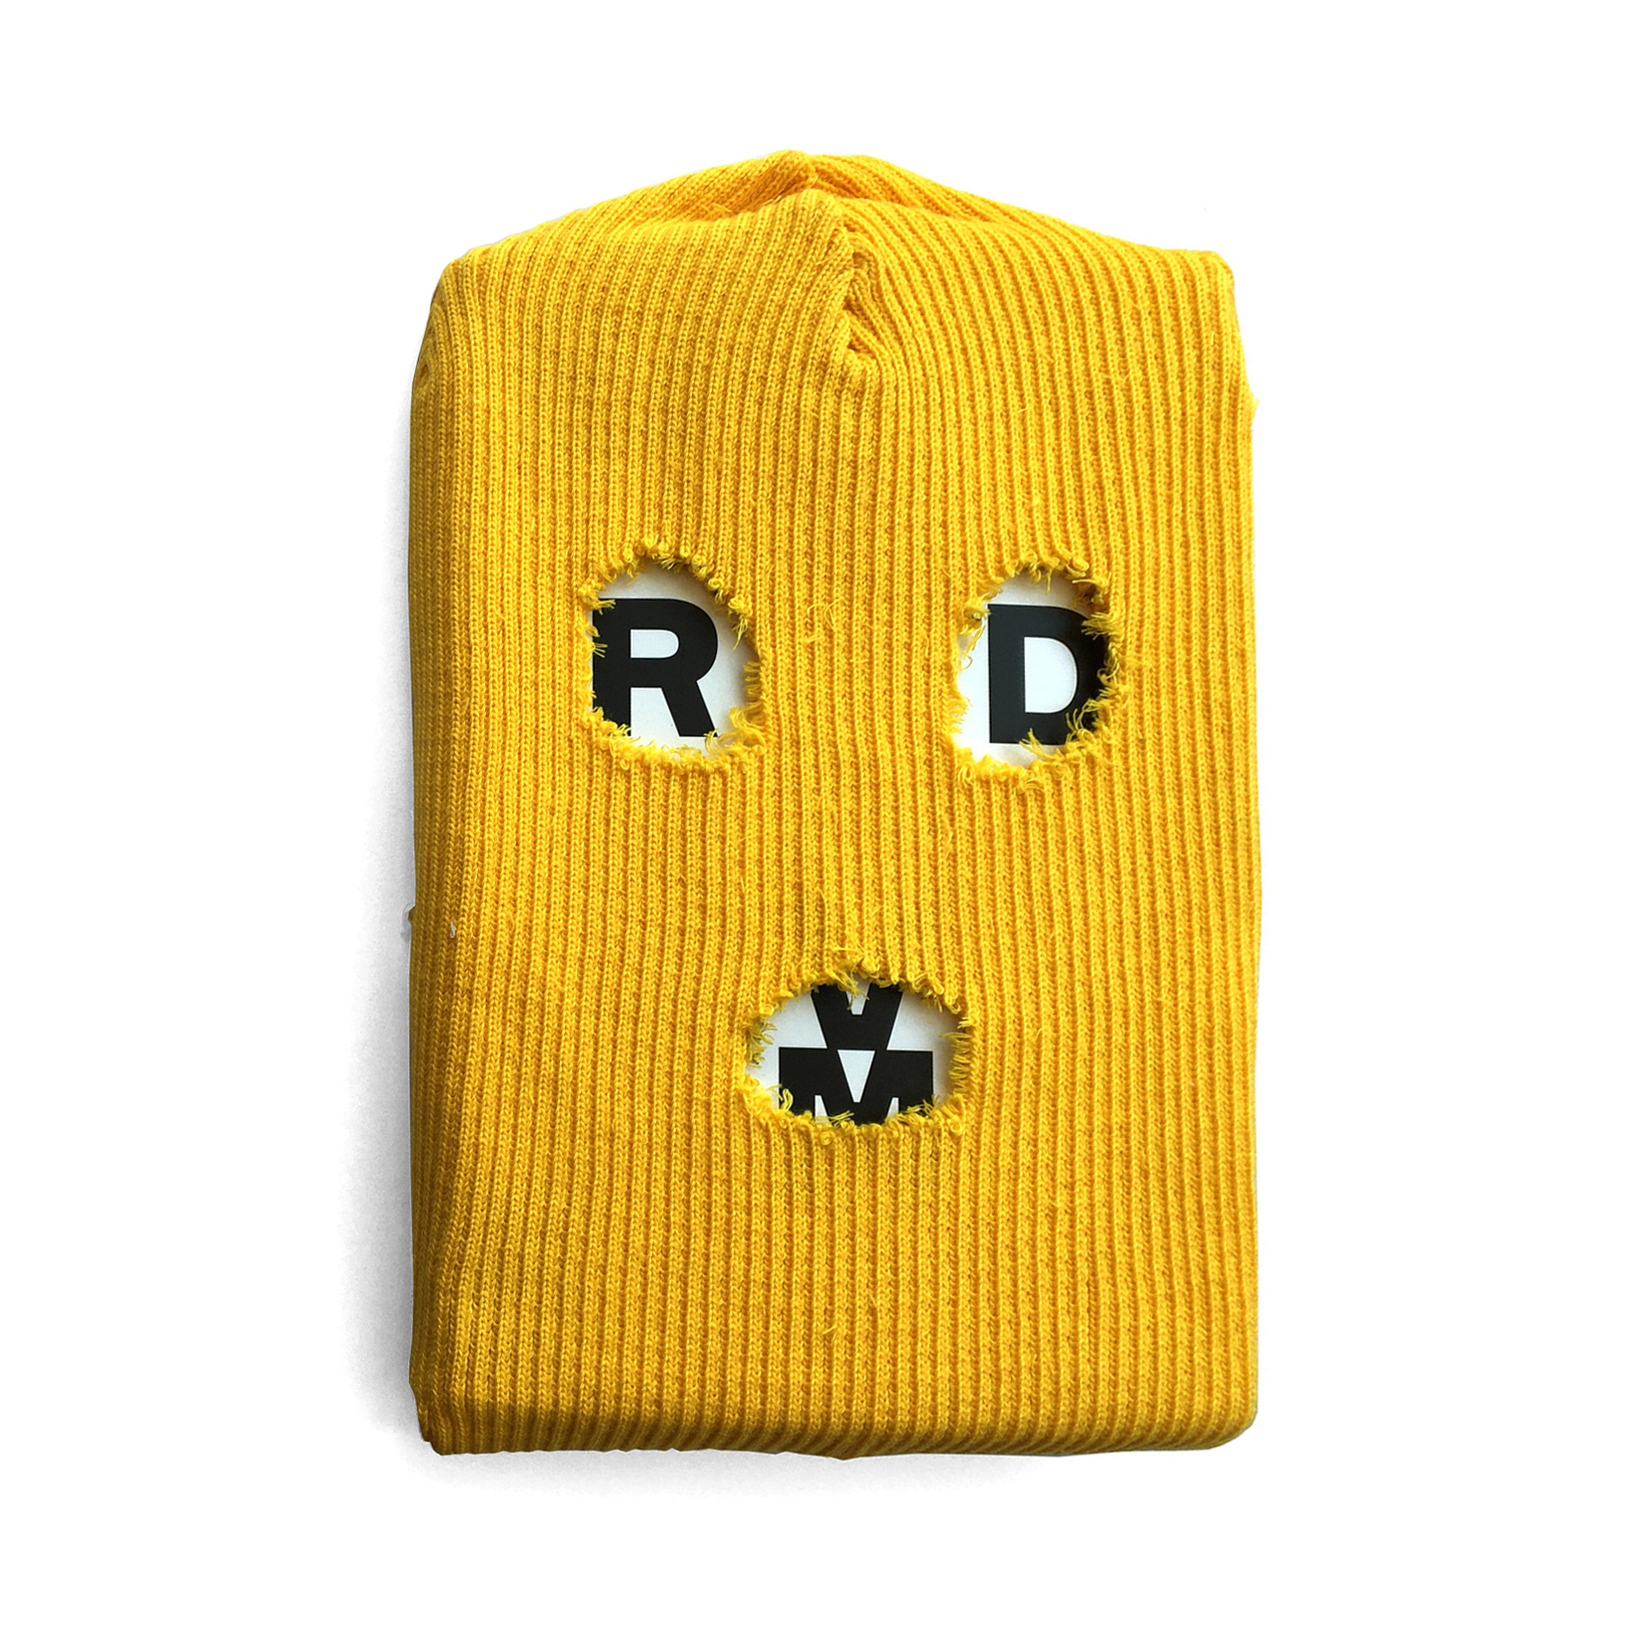
\includegraphics[width=74mm]{./grid/riot.jpg}
\end{center}

\hspace*{-7cm}\hrulefill\hspace*{-7cm}

\medskip

\noindent{}{\slsc{Nós somos Pussy Riot}} é um combo e também um libelo que se interpõe entre o patriarcado capitalista e encarcerador e as mulheres que ele vitimiza, de mais de uma forma: seu conteúdo é revolucionário, mas também o são as várias etapas de seu processo produtivo.

Ele é composto por \hlc[lightyellow]{``Riot days'', um relato cru, alucinatório e apaixonado sobre a prisão e julgamento de Maria Alyokhina em uma colônia penal nos Urais após participar junto com Pussy Riot, sua banda punk feminista, de um protesto punk contra Putin em uma igreja ortodoxa.}
E também de dois cordéis --- {\slsc{Sobre (Viver)}} e {\slsc{Engaiolaram"-nos}} --- tudo embalado em balaclavas coloridas, símbolo universal de resistência e luta social, confeccionadas especialmente pela Cooperativa Libertas, de mulheres egressas da máquina do sistema penitenciário brasileiro. Entre a banda Pussy Riot, perseguida em uma Rússia onde direitos das minorias são tolhidos, e as brasileiras que sofrem em um sistema desumano, há muito em comum. 

\vfill

\hspace*{-.4cm}\begin{minipage}[c]{.5\linewidth}
\small{
{\Formular{\textbf{
\hspace*{-.1cm}\hlc[lightyellow]{Editora: n-1 \& Hedra}\\
Título: Nós somos Pussy Riot\\
Autor: Maria Alyokhina\\ 
ISBN: 978-65-8109-713-4\\
Páginas: 216\\
Formato: 14x21cm\\
Preço: R\$ 89,90\\
Disponibilidade: Disponível
}}}}
\end{minipage}

\pagebreak %CORPOS QUE IMPORTAM, JUDITH BUTLER


\begin{center}
\hspace*{.5cm}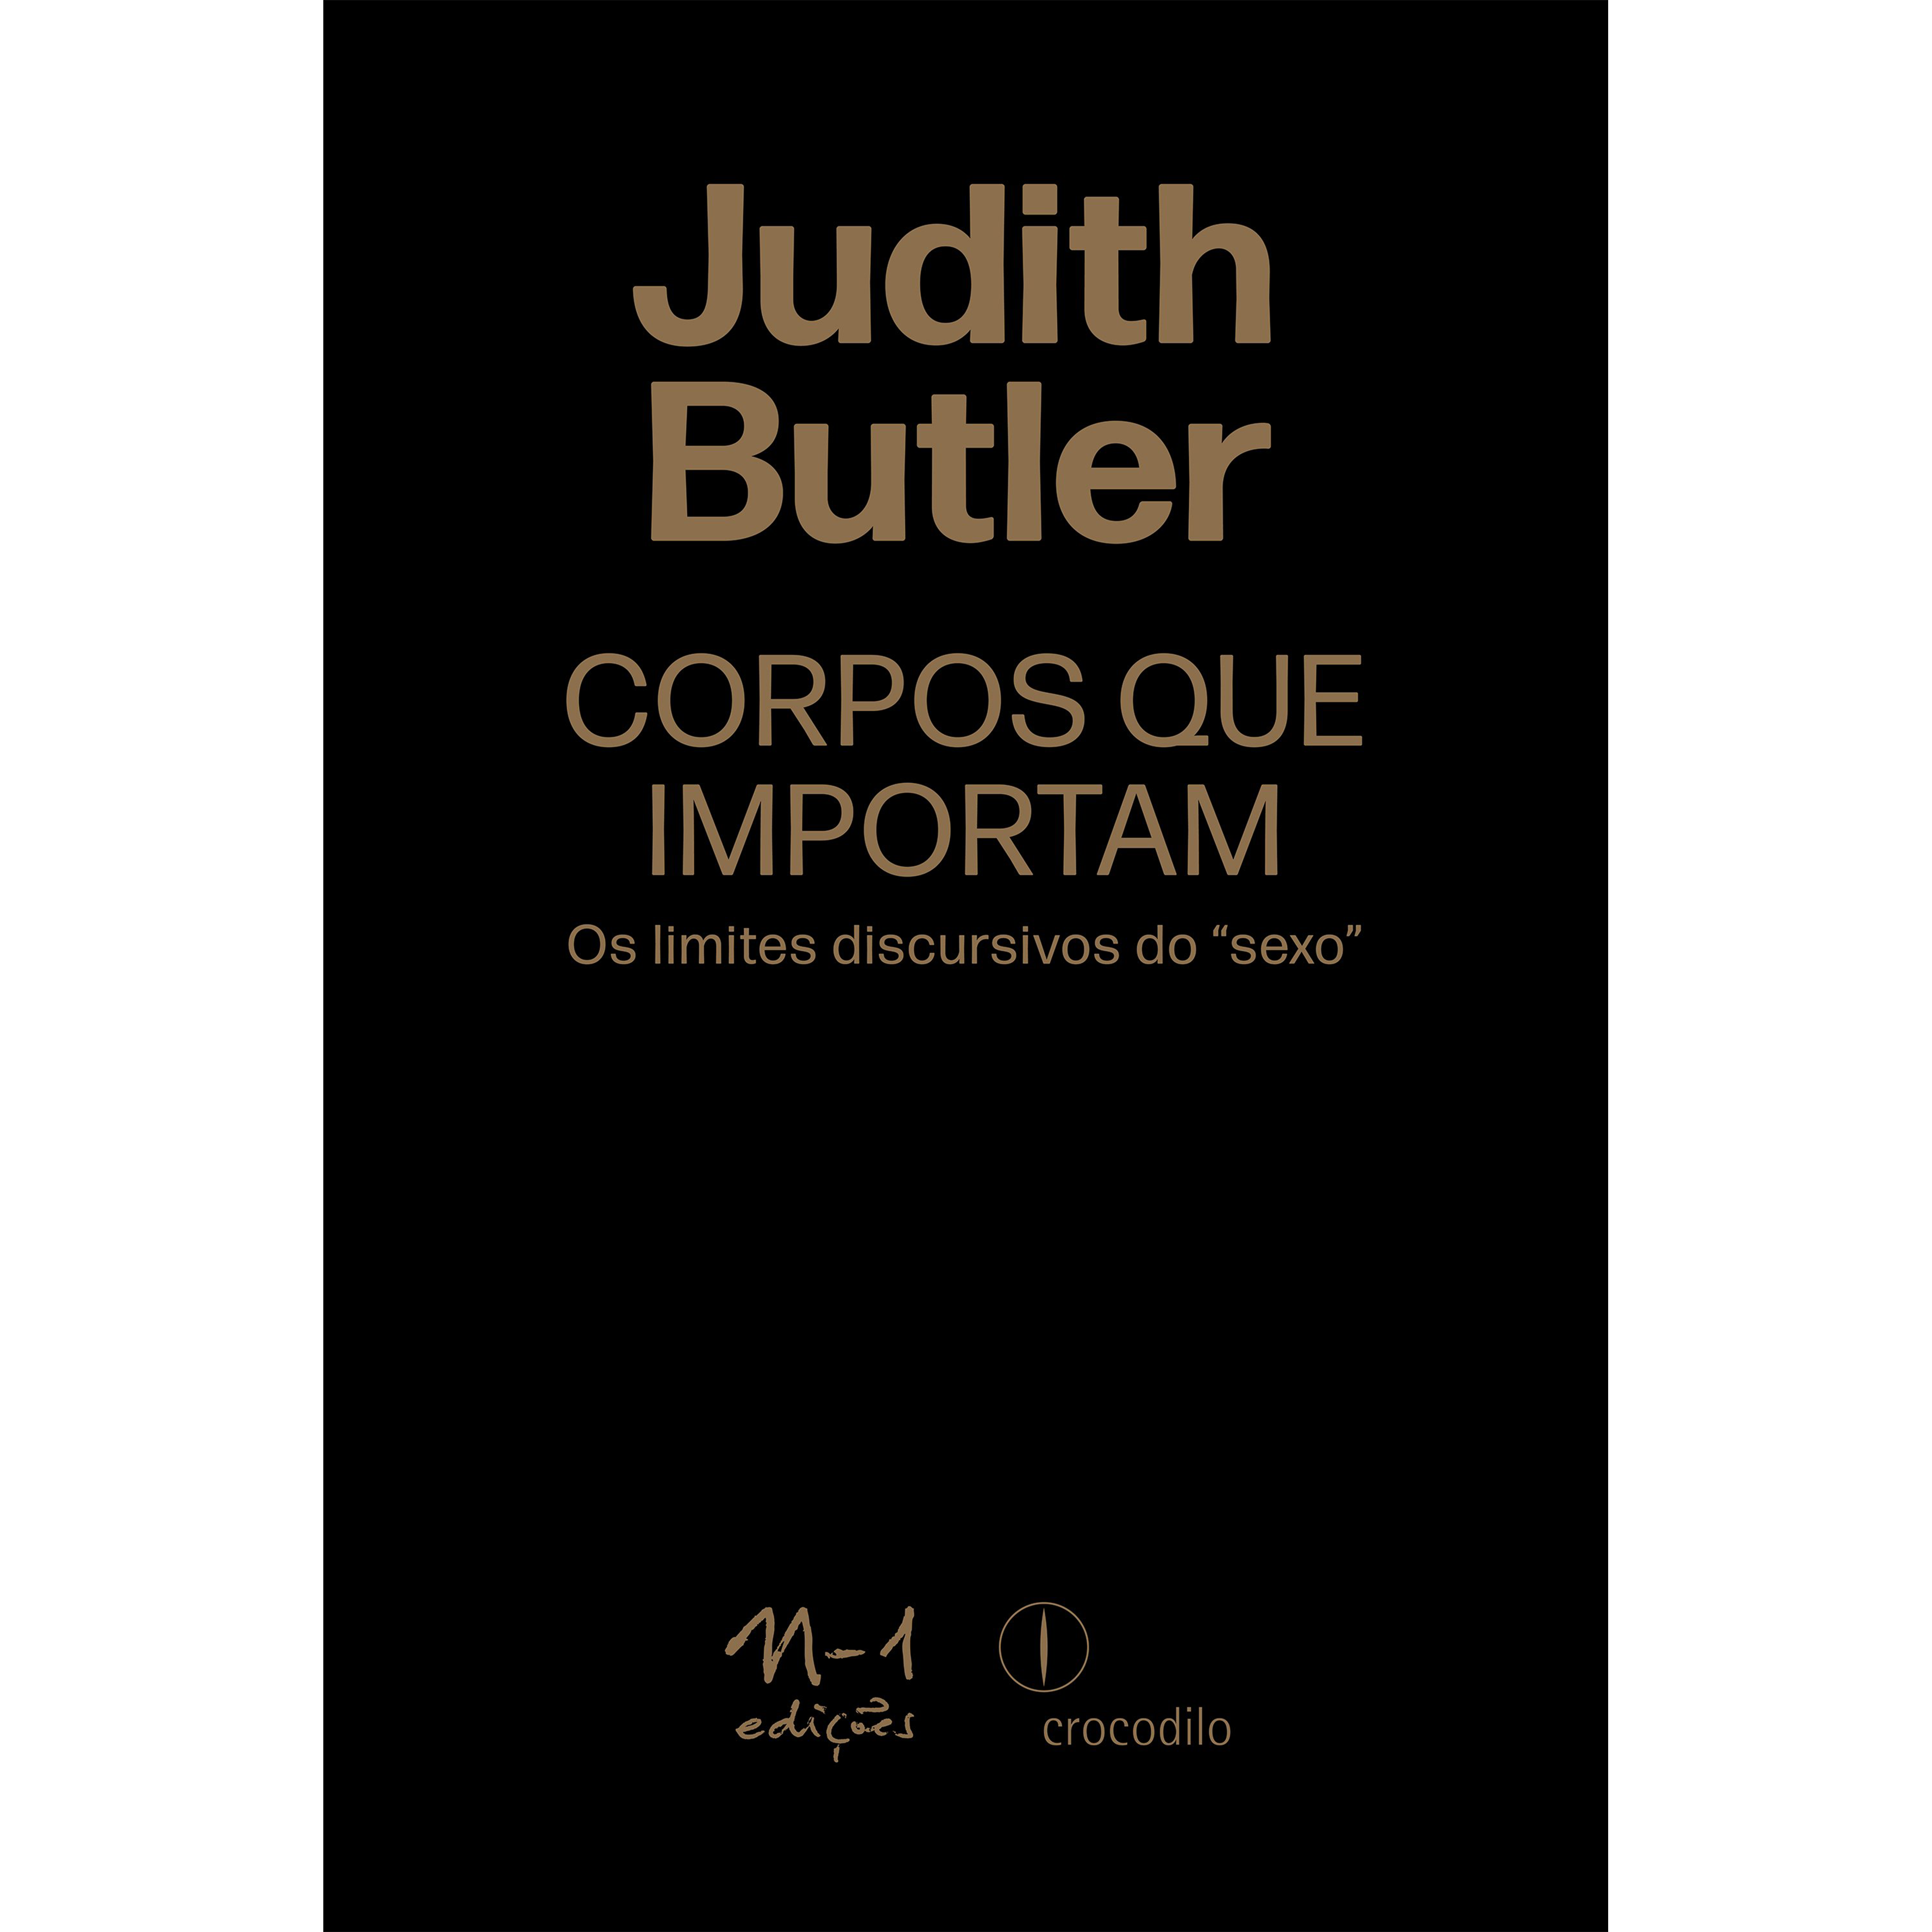
\includegraphics[width=74mm]{./grid/butler.png}
\end{center}

\hspace*{-7cm}\hrulefill\hspace*{-7cm}

\medskip

\noindent{}\hlc[lightyellow]{``Corpos que importam'' é sobre pensar a hegemonia heterossexual na criação de matérias [``matter''] sexuais e políticas.} Quais são as limitações pelas quais corpos são materializados como “sexuados”? E como devemos entender a “questão” [{\slsc{matter}}] do sexo e dos corpos de modo mais geral, como a circunscrição repetida e violenta da inteligibilidade cultural? Quais corpos importarão [{\slsc{matter}}] --- e por quê?

Nas palavras da filósofa pós"-estruturalista Judith Butler: “Ofereço este texto em parte como forma de reconsiderar algumas seções de meu livro {\slsc{Problemas de gênero}} que causaram confusão, mas também como um esforço para pensar mais sobre o funcionamento da hegemonia heterossexual na criação de matérias [{\slsc{matter}}] sexuais e políticas. Como uma rearticulação crítica de práticas teóricas, incluindo estudos feministas e {\slsc{queer}}, esta obra não pretende ser programática. E ainda como tentativa de esclarecer minhas “intenções”, ela também parece destinada a produzir novos conjuntos de mal"-entendidos. Espero que, ao menos, eles se provem produtivos.”


\vfill

\hspace*{-.4cm}\begin{minipage}[c]{1\linewidth}
\small{
{\Formular{\textbf{
\hspace*{-.1cm}\hlc[lightyellow]{Editora: n-1 \& Crocodilo}\\
Título: Corpos que importam – os limites discursivos do “sexo”\\
Autor: Judith Butler\\ 
ISBN: 978-65-8109-704-2\\
Páginas: 400\\
Formato: 14x21cm\\
Preço: R\$ 98,00\\
Disponibilidade: Disponível
}}}}
\end{minipage}

\pagebreak

\vspace*{1.5cm}

\noindent{}{\nohyphens{\LARGE{Traços humanos nas\\ superfícies do mundo}}}

\bigskip

\hfill\scalebox{.8}{JUDITH BUTLER}

\bigskip
\bigskip
\bigskip

\begin{multicols}{2}
Se antes não sabíamos que partilhamos as superfícies do mundo, o sabemos
agora. A superfície que uma pessoa toca carrega o traço dessa pessoa,
hospeda e transfere esse traço, afeta a próxima pessoa cujo toque pousa
ali. As superfícies diferem. O plástico não carrega o traço por muito
tempo, mas alguns materiais porosos claramente o carregam. Algo humano e
viral perdura breve ou demoradamente nessa superfície que constitui um
dos componentes materiais do nosso mundo comum.

Se não sabíamos o quão importante eram os objetos no vínculo de um ser
humano com outro, provavelmente o sabemos agora. A produção, reprodução
e consumo de bens carregam agora o risco de comunicar o vírus. Uma
encomenda é deixada na porta de casa, os traços do outro que a deixou
ali são invisíveis. Ao pegá"-la e trazê"-la para dentro, faz"-se contato
com esse traço e com muitos outros que não se sabe. A trabalhadora que
deixou a encomenda ali também carrega os traços de quem fez e empacotou
o objeto, de quem manuseou a comida. A trabalhadora é um local muito
especial de transmissão, assumindo o risco que aqueles que pedem comida
em casa procuram evitar. Embora a inter"-relação de todas essas pessoas
não seja visível, essa invisibilidade não nega sua realidade.
O objeto é
uma forma social, isto é, uma forma constituída por um conjunto de
relações sociais. Isso pode muito bem ser uma verdade geral, mas adquire
um novo significado sob as condições pandêmicas: por que o entregador de
comida ainda está trabalhando mesmo que isso o exponha mais prontamente
ao vírus do que alguém que recebe a comida por encomenda? Muitas vezes,
a escolha enfrentada por ele é a do risco da doença, possivelmente da
morte, ou de perder o emprego. A escolha brutal que a trabalhadora teve
que fazer dobra"-se também no traço humano que o objeto carrega, um traço
de trabalho que agora comporta potencialmente um traço do vírus. O vírus
não pertence a nenhum corpo que o contrai. Não é uma posse e nem um
atributo, ainda que digamos ``fulano ou ciclano {\slsc{tem}} o vírus''.
Pelo contrário, o vírus chega de outro lugar, submete a pessoa ao seu
jugo, transfere"-se para um orifício ou uma superfície corpórea pelo
toque ou pela respiração, toma o corpo como hospedeiro, escava"-o, entra
nas células e dirige sua replicação, estendendo seus filamentos letais,
tudo isso para penetrar no ar e derramar"-se sobre novas superfícies e
entrar em novas criaturas vivas. O vírus pousa, entra
\begin{wrapfigure}[7]{r}[.5\width+.5\columnsep]{5cm}
{\large
O objeto conecta pessoas de modos invisíveis, às
vezes indecifráveis; pessoas são interconectadas e não apenas
indivíduos isolados
}
\end{wrapfigure} nas fronteiras
corporais e parte para pousar novamente em outra pele ou em um objeto,
em busca de um hospedeiro --- a superfície de uma encomenda, o material
poroso de um mundo compartilhado. Os objetos que delineiam nossas
relações sociais são, por vezes, bens, mas, por outras, são corrimãos e
plataformas e todos os planos táteis da arquitetura da vida, o assento
de um avião, qualquer superfície que hospeda e transporta um traço por
mais que um momento passageiro. Nesse sentido, as superfícies do mundo
nos conectam, no limite elas estabelecem que somos igualmente
vulneráveis ao que atravessa as infraestruturas materiais e que
participa da superfície viva das coisas, e nos tornamos mais
perigosamente suscetíveis ao que vive nos objetos que nos entremeiam.
Dependemos dos objetos para viver, mas há por vezes também algo vivo no
objeto, ou um traço vivo de um outro ser humano na forma e na superfície
do objeto. A porosidade da superfície determina a longevidade e a
atividade do vírus, e, assim, as superfícies nas quais o vírus consegue
habitar sustentam sua vida. Como se sabe, nós humanos dependemos de um
mundo material para estabelecer o equilíbrio e o movimento, para prover
o ar que nos mantém respirando, e, dessa maneira, somos subitamente reduzidos  aos rudimentos da vida,
\begin{wrapfigure}[7]{l}[.5\width+.5\columnsep]{5cm}\end{wrapfigure}

\noindent{}deliberando a cada passo dado para
cumprir seus requisitos mais básicos. Em grande parte, as pessoas
parecem temer o contato próximo, cara a cara, a via aérea do vírus.O
encontro facial talvez seja ainda mais temido do que a contaminação pelo
objeto manuseado, e agora parece que a transmissão pelo ar é a forma
preponderante. Raramente temos controle total da nossa proximidade com
os outros no curso diário da vida: o mundo social é, nesse sentido,
imprevisível. A proximidade indesejada de objetos e de outras pessoas é
uma característica da vida pública e parece normal a qualquer um que
pega transporte público e que precisa se deslocar pela rua de uma cidade
densamente povoada: nós esbarramos uns nos outros em espaços estreitos,
nos apoiamos nos corrimãos, tocamos qualquer coisa que estiver pelo
caminho. E, no entanto, é essa condição de contato e de encontro ao
acaso, de roçar uns nos outros ou em qualquer coisa nos rodeando, que se
tornou potencialmente fatal, uma vez que o contato aumenta a
possibilidade da doença, e a doença traz consigo a possibilidade da
morte. Sob essas condições, os objetos e os outros dos quais
necessitamos aparecem potencialmente como as maiores ameaças às nossas
vidas.

As condições da pandemia nos impelem a reconsiderar como os objetos
estruturam e sustentam nossas relações sociais, encapsulando as relações
de trabalho, mas também as condições de vida e morte que o trabalho, o
movimento, a sociabilidade, o abrigo, implicam. Evidentemente, n´{\slsc{O
Capital}}, Marx nos detalha como o operariado investe seu trabalho no
objeto e como o valor do trabalho é transformado em valor de troca no
mundo socioeconômico estruturado pelo mercado. Ele procurou por
metáforas para descrever como o objeto manufaturado carrega e reflete o
traço do trabalho humano, e como o valor desse objeto, transformado em
mercadoria, é determinado pelo valor que os consumidores se dispõem a
pagar, pelo que os proprietários do lucro querem obter, e tudo isso
desemboca na noção de valor de mercado. O objeto foi ``mistificado'' e
``fetichizado'' precisamente porque incorporou um conjunto de relações
sociais de uma maneira enigmática. Nós não conseguiríamos olhar a
mercadoria sob uma ótica que iluminasse essas relações sociais com
transparência: elas eram embutidas no objeto de uma forma que
permaneceria misteriosa sem o tipo de análise proporcionada por Marx.
Nós tínhamos que entender o traço desaparecido de trabalho humano na
forma mercadoria junto com o animismo do objeto --- esse era um dos seus
efeitos mistificantes. Qualquer trabalho materializado em objeto era
praticamente suprimido pelo valor de troca deste objeto. O valor de
troca suprime do objeto o trabalho materializado qualquer que ele seja.
Apesar de sua negação pela forma mercadoria, o trabalho humano
sobrevivia como um traço invisível, não prontamente decifrável. Em
outras palavras, era um traço que demandava o tipo de leitura crítica
que Marx procurou oferecer. O fato de que as relações sociais sejam
coaguladas na forma de objeto não significa que essas relações, em sua
qualidade relacional, fossem boas ou justas. Dificilmente! Na verdade,
sob as condições do capital elas eram entendidas como relações tanto de
exploração como de alienação. E, no entanto, é essa mesma forma que
comunica também certos sinais de interdependência social. Uma cadeia de
trabalhadores, um sistema de trabalho, tudo entra na mercadoria de algum
jeito. A conclusão esperançosa que às vezes vem depois desse
{\slsc{insight}} toma forma assim: o objeto carrega o traço de humanos que
nós não conhecemos; o objeto conecta pessoas de modos invisíveis, às
vezes indecifráveis; logo, pessoas são interconectadas e não apenas
indivíduos isolados.

A tentação de regozijar"-se com a interconectividade deveria ser,
entretanto, rapidamente atenuada pelo reconhecimento de que estas formas
de interdependência podem estar imersas em condições de desigualdade e
exploração. Mesmo para Hegel, o \linebreak
\begin{center}
\begin{minipage}{13em}
{\large
Se perguntamos sobre a
forma geral do traço humano que a encomenda carrega, nós também estamos
perguntando sobre as condições de vida e morte que sustentam a
organização social do trabalho
}
\end{minipage}
\end{center}
precursor de Marx, ``o Senhor'' e ``o
Escravo'' são figuras interconectadas, interdependentes até, o que não
significa que sejam dependentes da mesma forma, ou que sejam igualmente
dependentes. Nem toda interdependência é recíproca. Ademais, cada um
negocia com a vida e a morte uma relação diferente. O Senhor busca
consumir o que o Escravo faz para a reprodução de sua própria vida, o
Escravo busca produzir o que o Senhor exige tendo em vista assegurar as
condições de sua própria vida --- condições que o Senhor controla. As
relações se condensam nessa forma. Mas será que a superfície carrega a
forma de maneira invisível? Não só a forma da superfície, mas a
superfície da forma. O corpo da trabalhadora jamais é totalmente
suprimido na forma mercadoria porque ela deixa alguns traços do seu
corpo no objeto, e também carrega, enquanto trabalha e vive, os traços
invisíveis de outras trabalhadoras.

Sob as condições de uma pandemia como a Covid"-19, trabalhar em e com
objetos de troca potencialmente dispara cargas de vírus letais. Por
regra, mesmo fora das condições de pandemia, se perguntamos sobre a
forma geral do traço humano que a encomenda carrega, nós também estamos
perguntando sobre as condições de vida e morte que sustentam a
organização social do trabalho. Quem arrisca sua vida enquanto trabalha?
Quem trabalhará até morrer? A mão de obra de quem é mal remunerada e,
então, dispensável e substituível? Sob as condições de uma pandemia
essas questões se intensificam. Entre as pessoas que são potencialmente
colocadas em risco ao fazer seus trabalhos estão servidores do sistema
de saúde trabalhando sem máscaras adequadas, empregados da Amazon sem
proteção e sobrecarregados, trabalhadores do serviço postal ou
entregadores {\slsc{delivery}} que não sabem se um traço letal é
transmitido por ou através deles conforme entregam encomendas e bens,
pessoas que vivem com tanto medo, mas que não podem se dar ao luxo de
perder esse emprego, pessoas que estão sem emprego e dependem da
distribuição pública de comida, aquelas pessoas para quem as ruas são o
chão e também o teto, aquelas abrigadas em condições aglomeradas e
perigosas, como prisões, ou albergues para indigentes, e aquelas que só
podem encontrar comida na rua.

Marx e Hegel fomentam um antropocentrismo segundo o qual a marca ou
traço humano anima o objeto com uma vitalidade especificamente humana. O
trabalhador tem a vida roubada pelo trabalho, mas a mercadoria emana uma
vida cada vez mais vibrante. E se o objeto que uma pessoa precisa é
também aquele que ameaça a vida dessa pessoa? Não o objeto sozinho, mas
o objeto manuseado, que carrega o traço do outro. O vírus atua na
superfície, mas a superfície também atua. O vírus entra no corpo, atua
nas células, se insere na ação das próprias células, para então atuar em
outros. Todas essas ações atuam quando o humano atua. O humano não é
mais que uma parte na cadeia de ações. Por sorte, o objeto não pode
transmitir o vírus se está coberto de sabão ou se sua superfície é
radicalmente não porosa. Então a porosidade do objeto contribui para a
transmissão; o objeto é definido, em parte, por sua porosidade: até o
ponto em que ele pode absorver ou carregar outro conjunto de materiais.
A porosidade é parte da definição tanto de humanos como de objetos; é
também uma outra forma de entender sua inter"-relação como potencial
interpenetrabilidade. ``Ficar em casa'' supostamente limita essa
porosidade, a possibilidade de o vírus ser transmitido entre humanos e
através de objetos e superfícies. No entanto, as pessoas que não têm
onde morar, vivendo sem abrigo, ou apenas em abrigo provisório, ou
aquelas forçadas por lei à quarentena em estruturas abarrotadas de gente
não podem manter o distanciamento social e não podem confiar na forma de
abrigo duradoura e segura que deve protegê"-las da exposição ao vírus.
Essa
\begin{center}
\begin{minipage}{13em}
{\large
A pandemia
intensifica a luta que opõe o capitalismo e suas desigualdades
sistêmicas, a destruição do planeta, a subjugação e a violência colonial
aos direitos dos sem"-teto e às minorias cujas vidas são
consideradas como não importantes
}
\end{minipage}
\end{center}
é apenas uma forma de desigualdade, de exposição e risco desiguais.
Aqueles que foram desprovidos de acesso a cuidados de saúde adequados
podem encontrar o vírus com sua imunidade comprometida, condições
médicas pré"-existentes. Não admira que, nos Estados Unidos, os
afro"-americanos tenham estatisticamente mais chance do que gente branca
de apresentar sintomas, de sofrer em maiores números, e de precisar de
hospitalização para sobreviver.


Na superfície, por assim dizer, a transmissão do vírus por meio de
objetos não tem nada que ver com a transmissão do valor do trabalho para
o valor de troca. Afinal de contas, o vírus parece trazer o mercado e as
finanças a um impasse. O mercado de ações despenca, os salários e as
poupanças são perdidos, os postos de trabalho subtraídos. Ao mesmo
tempo, entretanto, surge rapidamente um outro mercado para lucrar com a
pandemia. Muitos críticos sociais já publicaram textos sobre o
coronavírus e o capitalismo, abrindo um campo vital de pensamento e de
ativismo. Está em jogo saber se o capitalismo se aproveitará da pandemia
como uma nova oportunidade para a acumulação de riqueza para aqueles que
têm capital, ou se a pandemia vai pôr em xeque o capitalismo
desenfreado, lembrando"-nos da condição global que agora toca nossas
vidas. Enquanto alguns sustentam que as desigualdades se intensificarão
sob as condições da pandemia e o que se seguirá dela, outros sustentam
que as comunidades de cuidado que estão se organizando agora irão
despertar, ou darão novos contornos à potência do socialismo, à
solidariedade horizontal, e a uma genuína ética do cuidado. Fato é que
não sabemos. Quando o discurso público se volta para essa questão de
como o mundo recomeçará, podemos imaginar que o mundo será o mesmo (mas
cujas desigualdades se intensificarão) ou que será um mundo novo (no
qual reconheceremos nossa radical igualdade e interdependência). A minha
aposta é que o conflito entre essas duas visões se tornará mais
pronunciado. A continuação da emergência climática exige que se reduza a
produção, a extração, a perfuração, e os danos ambientais que cada vez
mais destroem os mundos"-de"-vida dos indígenas. O vírus coloca em
primeiro plano as diferenças raciais e geopolíticas do sofrimento, e
assistimos com claridade a resposta racista às condições da pandemia na
Índia, culpando a minoria muçulmana, o racismo contra asiáticos nos
Estados Unidos e na América Latina, e o fracasso intencional do Estado
Israelense de prestar assistência médica à Gaza, onde a população
palestina é contida à força em quarteirões estreitos com equipamentos de
saúde profundamente inadequados. A negligência intencional dos efeitos
letais da pandemia nas prisões é um tipo de assassinato por omissão.
Esta nova forma de sentença de morte não passa de mais um exemplo de
como a população encarcerada é vista como descartável, populações cujas
vidas não ``vale'' a pena salvar. Antes de mais nada, a pandemia
intensifica a luta que opõe o capitalismo e suas desigualdades
sistêmicas, a destruição do planeta, a subjugação e a violência colonial
aos direitos dos sem"-teto e da população encarcerada, das mulheres,
pessoas {\slsc{queer}} e trans, todas as minorias cujas vidas são
consideradas como não importantes. Ao mesmo tempo que está cada vez mais
evidente que uma vida vincula"-se a uma outra vida, e que esses vínculos
cruzam regiões, línguas e nações, que eles anunciam um comitê de
solidariedade global para o estabelecimento de condições dignas para
todas as vidas, está igualmente evidente que as desigualdades profundas
e intensas têm novas oportunidades de crescimento sob a pandemia.
Podemos predizer e profetizar na direção da utopia ou da distopia, mas
nada disso nos ajuda a firmar um ativismo contrário à obscena
distribuição de sofrimento em operação agora.

Sim, o vírus nos liga através de seus objetos e de suas superfícies,
através do encontro de perto com pessoas estranhas e íntimas,
confundindo e expondo os vínculos materiais que tanto condicionam como
põem em perigo a perspectiva da vida mesma. Mas essa igualdade perigosa
e potente é transfigurada em um mundo social e econômico onde se impõe
uma miríade de formas de desigualdade e uma demarcação notória das vidas
descartáveis. As comunidades de cuidado que construímos podem prefigurar
uma igualdade social por vir mais radical, mas se elas não ultrapassarem
as fronteiras de comunidades locais, línguas e nações, não veremos o
sucesso da tradução dos experimentos comunitários em uma política
global. As superfícies da vida ensinam aos humanos sobre o mundo que
compartilham, insistindo que estamos interconectados. Mas enquanto os
sistemas de saúde continuarem inacessíveis e impagáveis para tantas
pessoas, enquanto os ricos, os xenófobos, os racialmente privilegiados
persistirem com sua convicção arrogante de que serão os primeiros da
fila para qualquer vacina que surja, para o antiviral prometido, ou para
o acesso ao plasma repleto de anticorpos, aqueles laços serão quebrados
e arruinados, a desigualdade se intensificará. As consequências são
óbvias: a vida é um direito só dos privilegiados. O vírus não traz
consigo nenhuma lição moral; é uma angústia sem justificativa moral. E,
no entanto, nos oferece uma visão refratada de uma potente e
interconectada solidariedade global. Isso não ocorrerá por vontade
própria, mas apenas por meio de uma luta que se renova agora, durante o
{\slsc{lockdown}}, em nome da igualdade do vivente.\footnote[1]{Texto originalmente publicado no site da n-1 edições. Tradução de André Arias e Clara Barzaghi.}
\end{multicols}

\pagebreak %SOMOS NOSSO CÉREBRO?

\begin{center}
\hspace*{.5cm}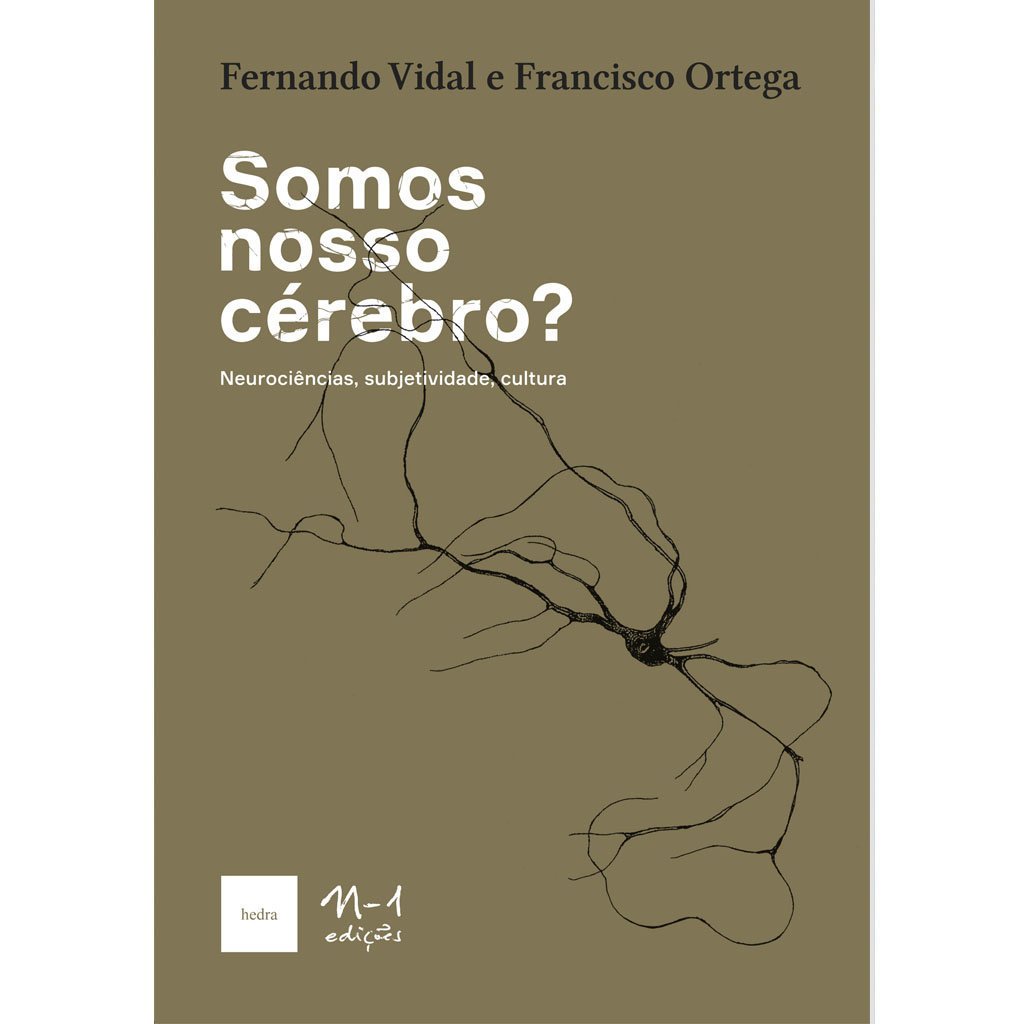
\includegraphics[width=74mm]{./grid/cerebro.png}
\end{center}

\hspace*{-7cm}\hrulefill\hspace*{-7cm}

\medskip

\noindent{}Explorando o neurocentrismo, a crença de que “somos nossos cérebros” se difundiu nos anos 1990. Encorajados pelos avanços da neuroimagem, as humanidades e as ciências sociais adotaram uma “virada neurocientífica” na forma de neuro"-subespecialidades em campos como antropologia, estética, educação, história, direito, sociologia e teologia. Empresas comerciais duvidosas, mas bem"-sucedidas, como “neuromarketing” e “neurobica” surgiram para tirar proveito da sensibilidade aumentada para todo o universo neuro.

Embora não seja hegemônica nem monolítica, a visão neurocêntrica encarna uma poderosa ideologia que está no cerne de alguns dos mais importantes debates filosóficos, éticos, científicos e políticos da atualidade. \hlc[lightyellow]{``Somos nosso cérebro?'' escolhido livro do ano em 2018 pela ``International Society for the History of the Neurosciences'', examina a lógica interna de tal ideologia, sua genealogia e suas principais encarnações contemporâneas.} 


\vfill

\hspace*{-.4cm}\begin{minipage}[c]{.5\linewidth}
\small{
{\Formular{\textbf{
\hspace*{-.1cm}\hlc[lightyellow]{Editora: n-1 \& Hedra}\\
Título: Somos nosso cérebro?\\ Neurociências, subjetividade, cultura\\
Autor: Francisco Ortega e Fernando vidal\\ 
ISBN: 978-65-9582-035-7\\
Páginas: 346\\
Formato: 16x23cm\\
Preço: R\$ 80,00\\
Disponibilidade: Disponível
}}}}
\end{minipage}

\pagebreak %PRAGMATISMO PULSIONAL


\begin{center}
\hspace*{-3.6cm}\raisebox{5cm}{\rotatebox[origin=t]{90}{\huge\Formular{\textbf{Lançamento}}}}
\hspace*{3.1cm}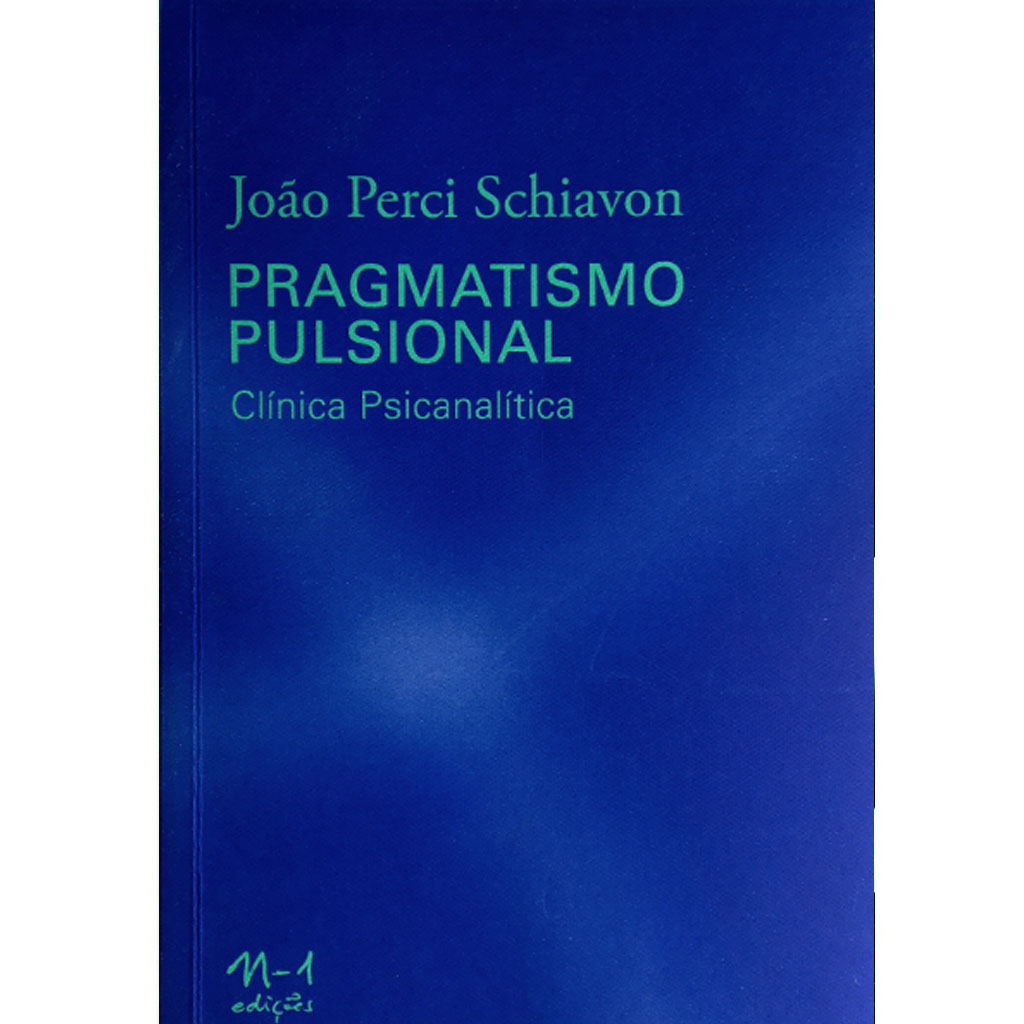
\includegraphics[width=74mm]{./grid/gozo.jpg}
\end{center}

\hspace*{-7cm}\hrulefill\hspace*{-7cm}

\medskip

\noindent{}Raros são os psicanalistas que têm tamanho domínio de Lacan e de Guattari a um só tempo, e que a exemplo de João Perci Schiavon, professor da \scalebox{.8}{PUC-SP} e autor de obras como {\slsc{A lógica da vida desejante}}, conseguem alcance clínico e filosófico de tal envergadura.  

A uma \hlc[lightyellow]{atmosfera de convite a experimentação do fluxo inconsciente e aposta clínica num diapasão em tudo singular entrecruza assuntos --- a contribuição freudiana à linhagem filosófica que vai de Nietzsche a Deleuze.} E a pulsão reaparece sob nova luz: o gozo, este que não serve a nenhum bem, engendra todos os bens possíveis e todas as utilidades, algo desconcertante se tivermos em vista o título do escrito, {\slsc{Pragmatismo pulsional}}.

O livro pode ser lido e vivido como “experiência” subjetiva, clínica, filosófica, micropolítica --- isto é, de transformação. O que mais se pode exigir de um livro hoje além de que faça diferença, e diferença para a vida? A pulsão é uma autoridade no que diz respeito ao vivo ou ao desejo. Ela só precisa ser exercida, e o nome desse exercício é cura.

\vfill

\hspace*{-.4cm}\begin{minipage}[c]{.8\linewidth}
\small{
{\Formular{\textbf{
\hspace*{-.1cm}\hlc[lightyellow]{Editora: n-1}\\
Título: Pragmatismo pulsional – clínica psicanalítica\\
Autor: João Perci Schiavon\\ 
ISBN: 978-65-8109-706-6\\
Páginas: 336\\
Formato: 14x21cm\\
Preço: R\$ 66,00\\
Disponibilidade: Disponível
}}}}
\end{minipage}

\pagebreak %FASCISMO OU REVOLUÇÃO? MAURICIO LAZZARATO


\begin{center}
\hspace*{.5cm}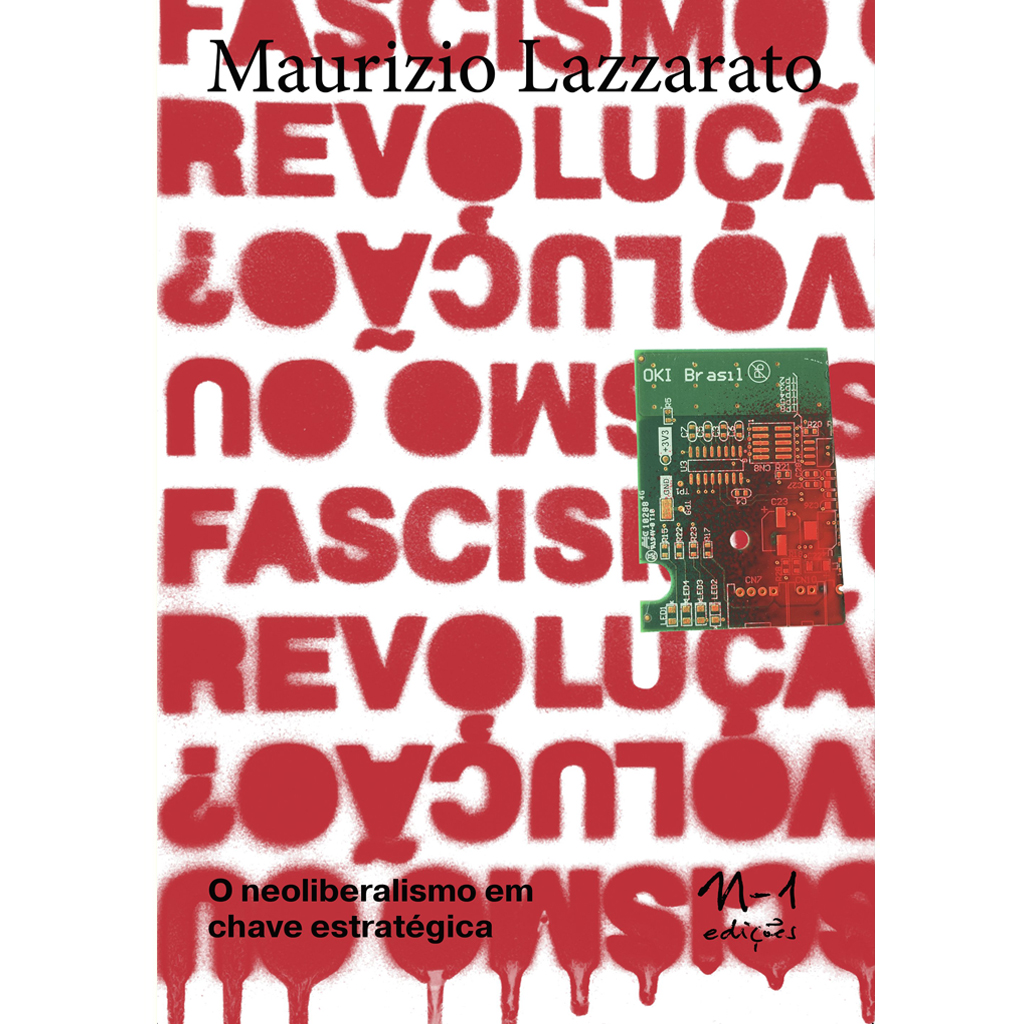
\includegraphics[width=74mm]{./grid/lazzarato.png}
\end{center}

\hspace*{-7cm}\hrulefill\hspace*{-7cm}

\medskip

\noindent{}O fascismo histórico foi tão moderno quanto o capitalismo (já que é uma de suas expressões), como demonstrado nitidamente pelo futurismo italiano. O mesmo ocorre com o novo fascismo, que é um ciberfascismo. Ele põe em xeque todas as utopias tecnociber (do ciberpunk ao ciberfeminismo, da ciberesfera à cibercultura) que desde o pós"-guerra, principalmente a partir dos anos 1970, viam nas máquinas cibernéticas uma dupla promessa: a de uma nova subjetividade pós"-humana e a da liberação da dominação capitalista, cuja ruptura viria das máquinas e não da política. Das revoluções da técnica e não da organização revolucionária.

\hlc[lightyellow]{Bolsonaro e Trump utilizaram todas as tecnologias disponíveis da comunicação digital, mas suas vitórias não vêm da tecnologia. São o resultado da máquina política e estratégia que agencia uma micropolítica dos afetos tristes} (frustração, ódio, inveja, angústia medo) com relação à macropolítica de um novo fascismo, que dá consistência política às subjetividades devastadas na financeirização.

\vfill

\hspace*{-.4cm}\begin{minipage}[c]{.5\linewidth}
\small{
{\Formular{\textbf{
\hspace*{-.1cm}\hlc[lightyellow]{Editora: n-1}\\
Título: Fascimo ou Revolução?\\
Autor: Mauricio Lazzarato\\ 
ISBN: 978-85-6694-381-8\\
Páginas: 208\\
Formato: 14x21cm\\
Preço: R\$ 69,00\\
Disponibilidade: Disponível
}}}}
\end{minipage}

\pagebreak %ESPAÇO CORUJA

\begin{center}
\hspace*{-3.6cm}\raisebox{5cm}{\rotatebox[origin=t]{90}{\huge\Formular{\textbf{Lançamento}}}}
\hspace*{3.1cm}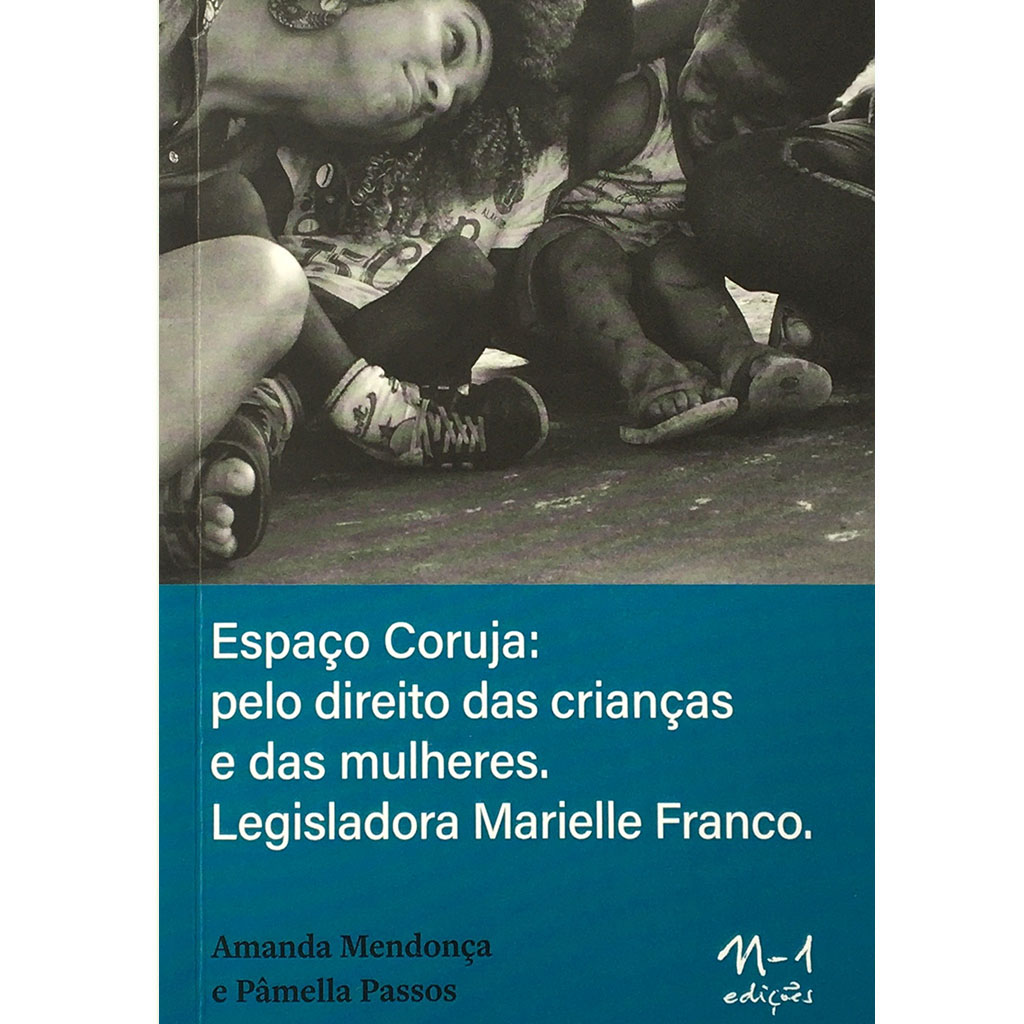
\includegraphics[width=74mm]{./grid/coruja.jpg}
\end{center}

\hspace*{-7cm}\hrulefill\hspace*{-7cm}

\medskip

\noindent{}\hlc[lightyellow]{“A formulação do Projeto de Lei do Espaço Coruja foi uma das ações de maior impacto emocional para Marielle. Era a sua história: uma mulher negra, favelada, que foi mãe jovem e precisava de um lugar seguro para deixar sua filha enquanto trabalhava e estudava.} Ela teve uma rede de familiares e de amigos que lhe garantiu avançar e concluir seus estudos. Mas conhecia as diversas e duras realidades da maioria das mulheres que não possuem essa oportunidade. Com empatia e olhar solidário, ela propôs, como legisladora, a criação do Espaço Infantil Noturno. Foram muitos os momentos em que a vi preocupada e empenhada com a elaboração desse projeto tão caro a ela. Ouvinte ativa às críticas, sempre buscou ponderar, mas tinha em seu próprio corpo e história de vida a certeza da urgência. Com essa lei, crianças terão direito a um lugar seguro enquanto suas mães e pais trabalham e/ou estudam --- em um mundo mais justo e igualitário e movimentando as estruturas dessa sociedade ainda tão patriarcal, misógina, machista e racista.” [Mônica Benício]


\vfill

\hspace*{-.4cm}\begin{minipage}[c]{1\linewidth}
\small{
{\Formular{\textbf{
\hspace*{-.1cm}\hlc[lightyellow]{Editora: n-1}\\
Título: Espaço Coruja: pelo direito\\ das crianças e das mulheres\\
Autor: Amanda Mendonça e Pâmella Passos\\ 
ISBN: 978-65-8109-705-9\\
Páginas: 64\\
Formato: 10x16cm\\
Preço: R\$ 20,00\\
Disponibilidade: Disponível
}}}}
\end{minipage}

\pagebreak %UM PIANO NAS BARRICADAS, TARÌ

\begin{center}
\hspace*{.5cm}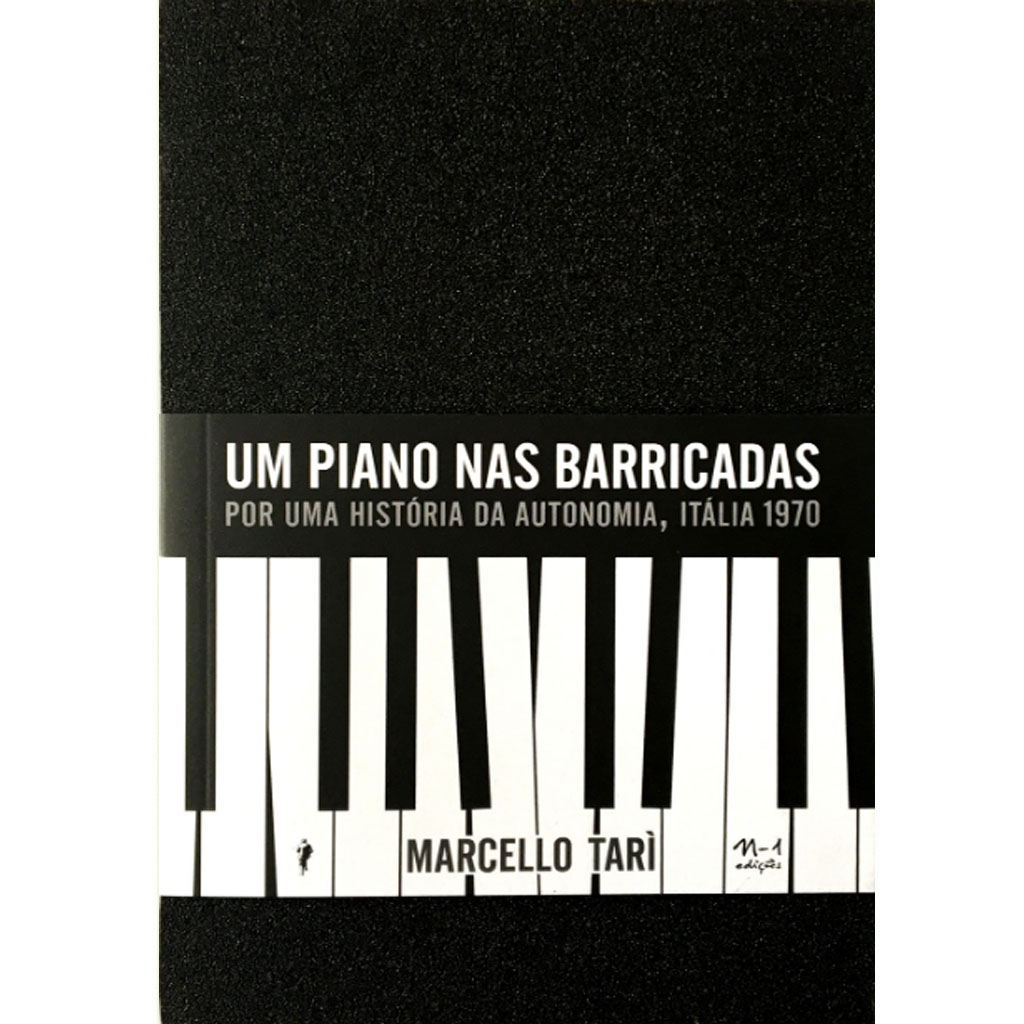
\includegraphics[width=74mm]{./grid/barricada.png}
\end{center}

\hspace*{-7cm}\hrulefill\hspace*{-7cm}

\medskip

\noindent{}Nos filmes sociais e políticos dos anos 1970 na Itália, a Autonomia é apresentada como um método intermediário entre Marx e a antipsiquiatria, a Comuna de Paris e a contracultura, o dadaísmo e o insurrecionalismo, o operaísmo e o feminismo e muitas coisas com outras coisas. Mas apresentou acima de tudo descontinuidade profunda com a prática do Movimento Operário oficial. Não era e nunca foi uma organização, mas uma multiplicidade que se organizava a partir de onde residiam, trabalhavam ou estudavam os sujeitos que a deram forma.

Na Autonomia, muitas autonomias específicas surgiram e coexistiram: operários, estudantes, mulheres, homossexuais, prisioneiros --- ou de qualquer um que escolhesse, a partir de suas próprias contradições, o caminho da luta por um modo reluzente de subversão da vida contra o trabalho assalariado e o Estado. \hlc[lightyellow]{Se o Movimento dos anos 1970 acabou sucumbindo às forças combinadas da máquina estatal e do Partido Comunista, a história da autonomia destaca"-se desse contexto, pois é a de uma aventura revolucionária cuja incandescência atual é mais relevante do que nunca.} 

\vfill

\hspace*{-.4cm}\begin{minipage}[c]{1\linewidth}
\small{
{\Formular{\textbf{
\hspace*{-.1cm}\hlc[lightyellow]{Editora: n-1 \& Glac}\\
Título: Um piano nas barricadas – por uma história da autonomia\\
Autor: Marcelo Tarì\\ 
ISBN: 978-65-8042-104-6\\
Páginas: 384\\
Formato: 12x19cm\\
Preço: R\$ 80,00\\
Disponibilidade: Disponível
}}}}
\end{minipage}

\pagebreak %FAVARRETO


\begin{center}
\hspace*{-3.6cm}\raisebox{5cm}{\rotatebox[origin=t]{90}{\huge\Formular{\textbf{Lançamento}}}}
\hspace*{3.1cm}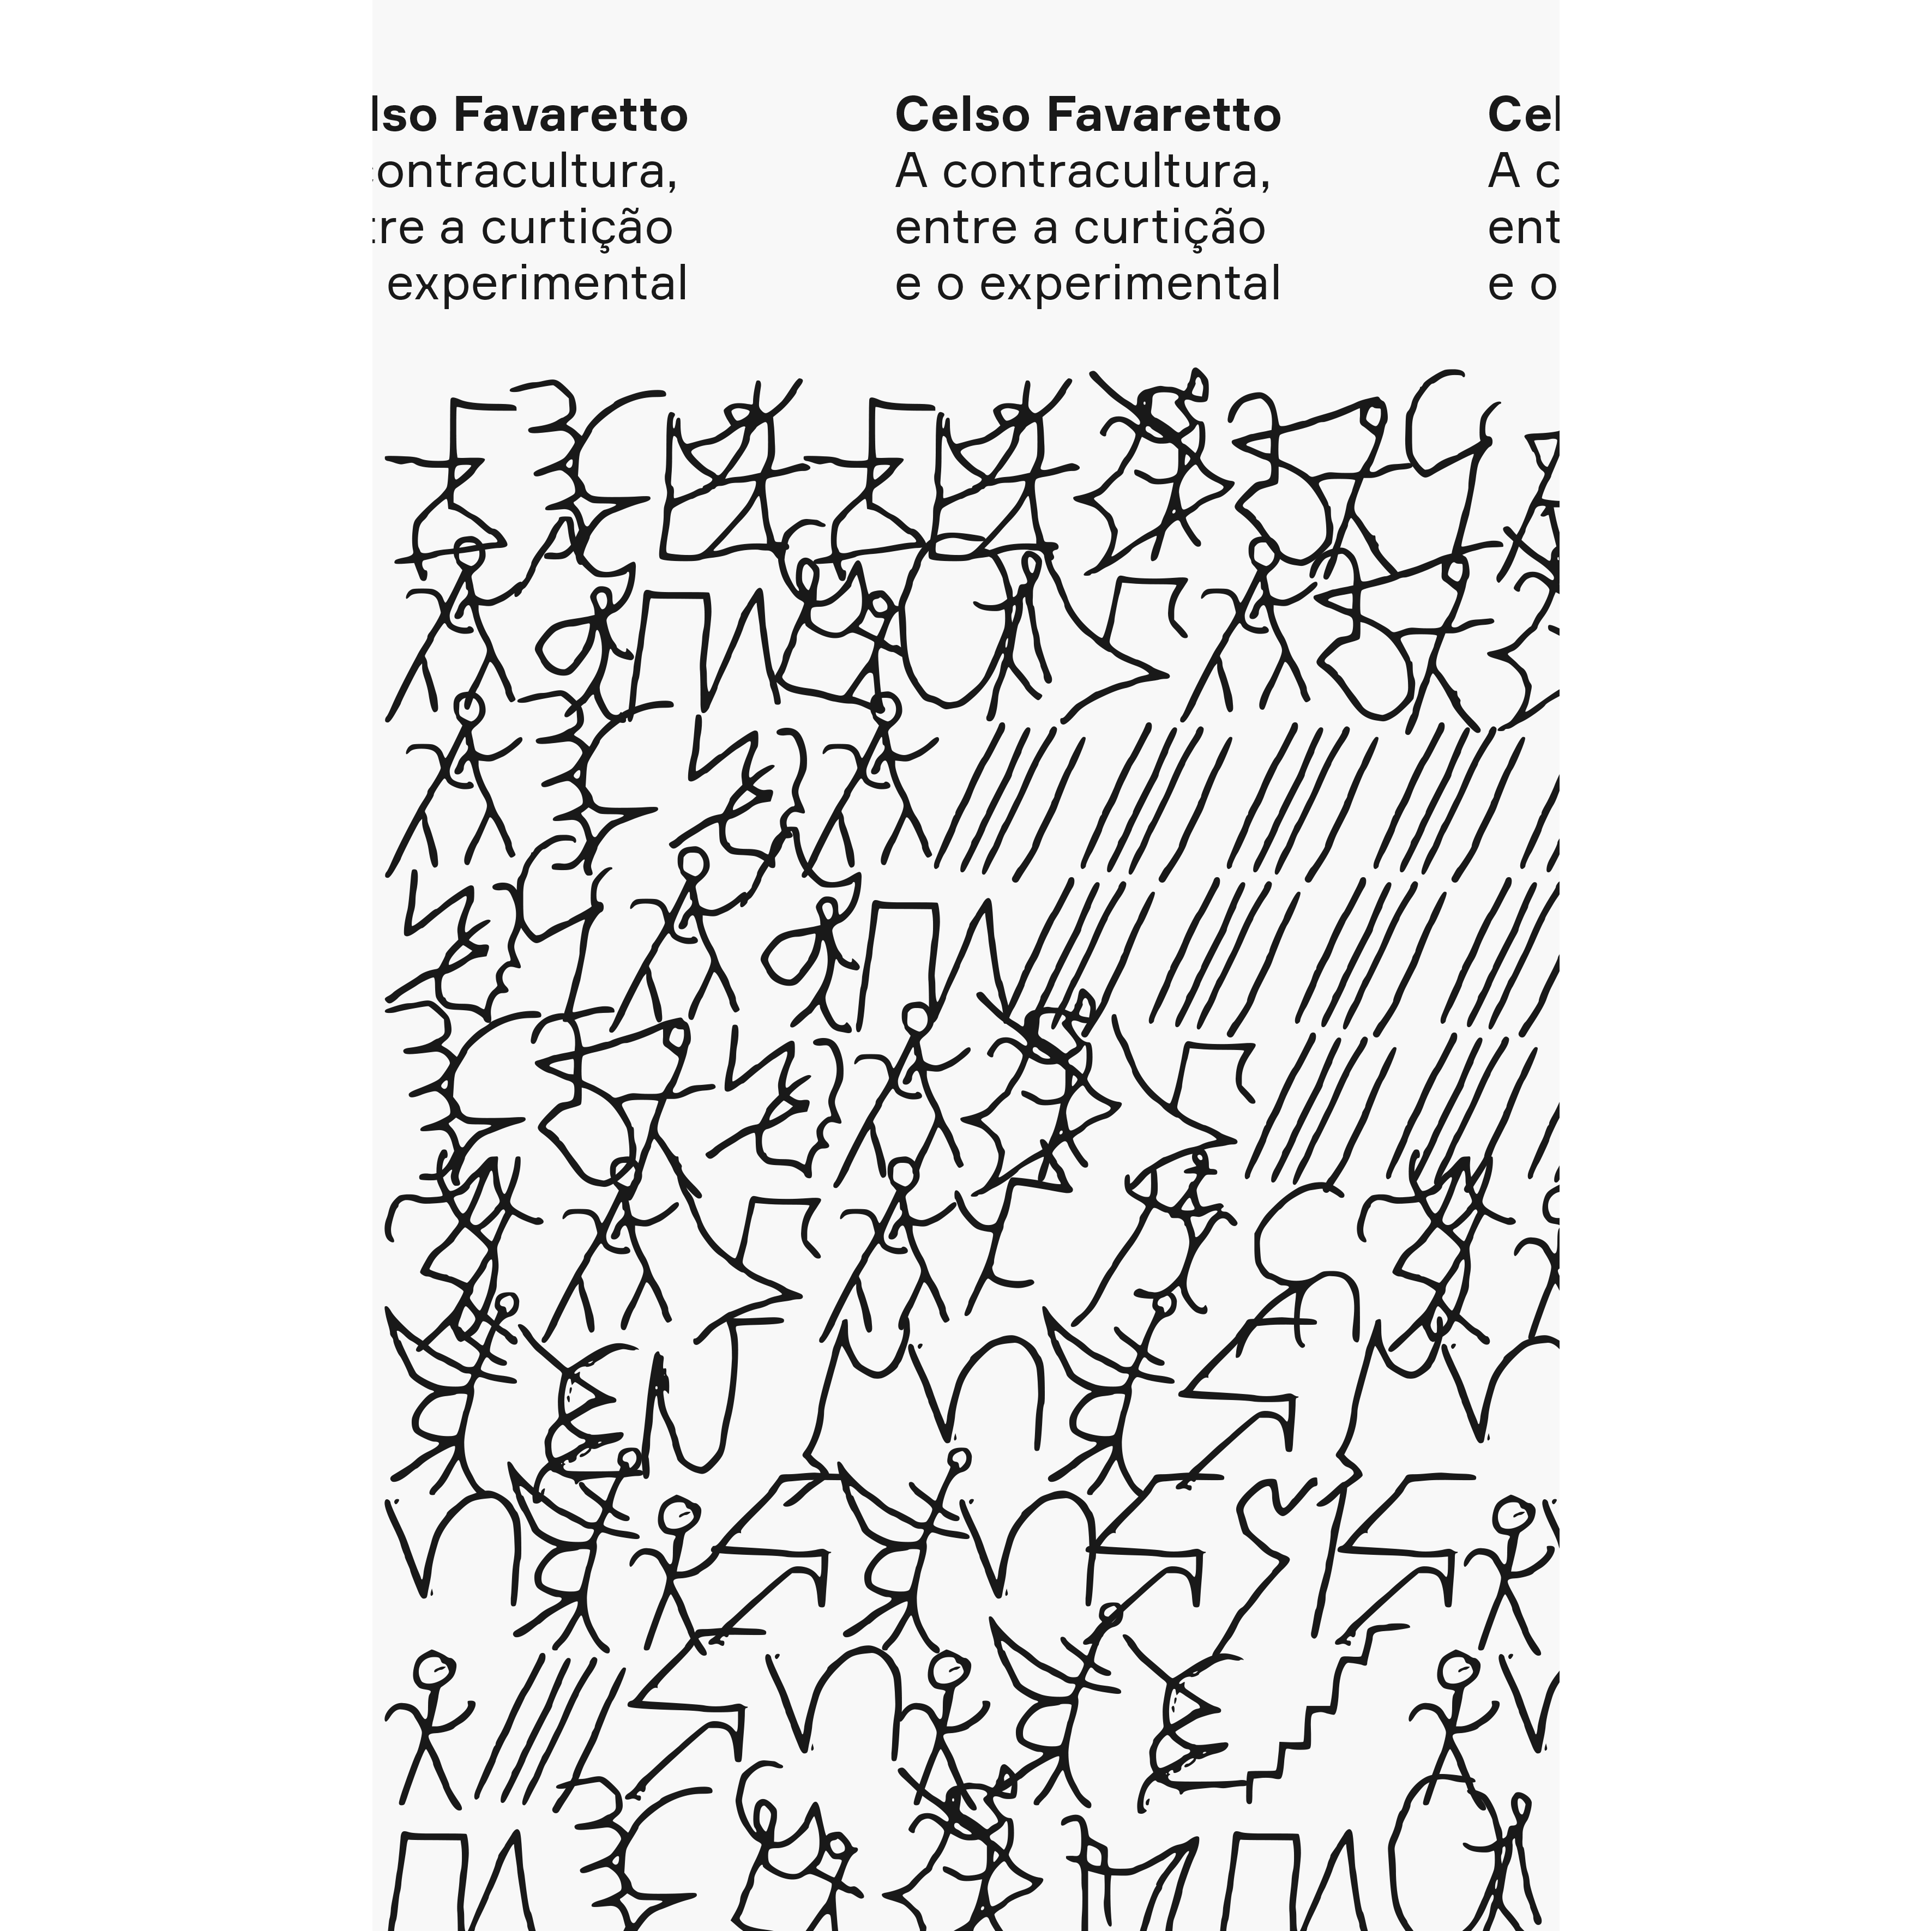
\includegraphics[width=74mm]{./grid/favaretto.png}
\end{center}

\hspace*{-7cm}\hrulefill\hspace*{-7cm}

\medskip

\noindent{}Neste livro o pesquisador e intelectual Celso Favaretto aborda as manifestações contraculturais que marcaram a produção artística brasileira entre os anos 60 e 70. Manifestava"-se então uma nova sensibilidade às margens da política oficial e da indústria cultural, expressa em experimentações artísticas com diversas possibilidades abertas pelo tropicalismo. \hlc[lightyellow]{Longe de um suposto “vazio cultural”, a contracultura por variadas expressões definiu atitudes, comportamentos, gestos exemplares, experimentações de grande vitalidade.} Inclusive, em alguns casos, a resistência às limitações da cultura oficial e à repressão da ditadura.

Composto por três ensaios, são revisitados no livro importantes personalidades e eventos da cultura brasileira --- como Caetano Veloso, Waly Salomão, Glauber Rocha, Zé Celso e o Teatro Oficina, Augusto Boal, Antonio Callado, José Agrippino de Paula, Hélio Oiticica --- sincrônicos aos desdobramentos políticos e sociais implicados pelo Golpe Civil"-Militar.

\vfill

\hspace*{-.4cm}\begin{minipage}[c]{.5\linewidth}
\small{
{\Formular{\textbf{
\hspace*{-.1cm}\hlc[lightyellow]{Editora: n-1 \& Hedra}\\
Título: A contracultura, entre\\ a curtição e o experimental\\
Autor: Celso Favaretto\\ 
ISBN: 978-65-8109-703-5\\
Páginas: 142\\
Formato: 11x18cm\\
Preço: R\$ 40,00\\
Disponibilidade: Disponível
}}}}
\end{minipage}

\pagebreak %RITORNELOS

\begin{center}
\hspace*{.5cm}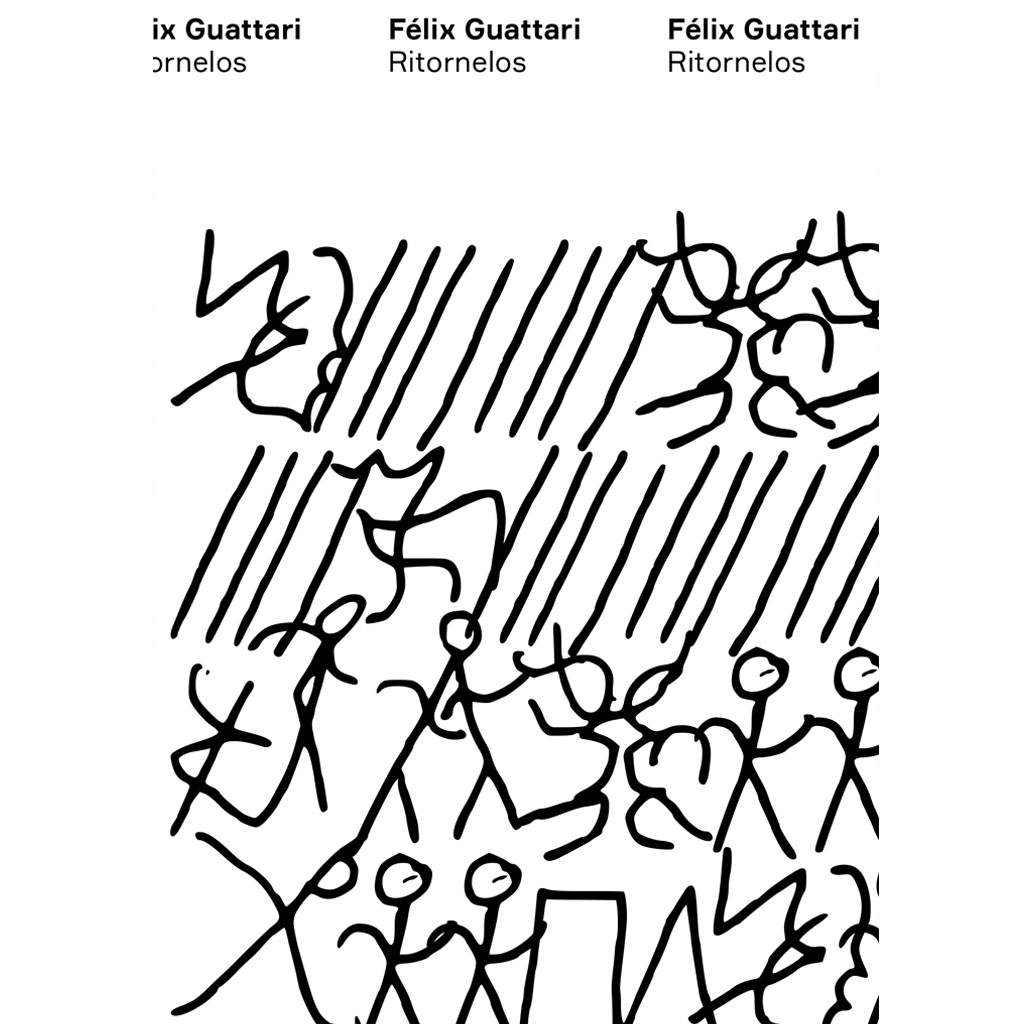
\includegraphics[width=74mm]{./grid/guattari.jpg}
\end{center}

\hspace*{-7cm}\hrulefill\hspace*{-7cm}

\medskip

\noindent{}Livro póstumo do pensador e psicanalista francês Félix Guattari, {\slsc{Ritornelos}} é uma obra inclassificável. \hlc[lightyellow]{Misto de poesia, relatos autobiográficos, ``frames'' do cotidiano, toda potência da escrita esquiza irrompe nessas páginas de alta voltagem poética e imagética.} Além de arguto intelectual, Guattari aparece em {\slsc{Ritornelos}} enquanto poeta sensível aos instantâneos e surreais quadros da vida.

Ao longo de suas páginas, vemos a fluidez com que a escrita de Guattari escorre sobre a superfície da vida, penetra em suas estruturas fragmentadas e as transporta ao seu revés. Através desse torvelinho de imagens decompostas o livro leva o leitor a percorrer o universo único do filósofo: cenas de amor e intimidade, de amizades, captadas nas ruas e praças parisienses, suas referências literárias e cinematográficas, quase em um mapeamento afetivo e cartográfico do autor de {\slsc{O anti-Édipo}}. Publicado somente nos anos 2000 na França, é a primeira vez que o livro é traduzido e editado no Brasil, em trabalho minucioso de tradutor"-ourives para acompanhar todas as nuances, rupturas e labirintos do texto original.

\vfill

\hspace*{-.4cm}\begin{minipage}[c]{.5\linewidth}
\small{
{\Formular{\textbf{
\hspace*{-.1cm}\hlc[lightyellow]{Editora: n-1 \& Hedra}\\
Título: Ritornelos\\
Autor: Félix Guattari\\ 
ISBN: 978-65-8109-702-8\\
Páginas: 134\\
Formato: 11x18cm\\
Preço: R\$ 40,00\\
Disponibilidade: Disponível
}}}}
\end{minipage}

\pagebreak


\begin{center}
\hspace*{-3.6cm}\raisebox{5cm}{\rotatebox[origin=t]{90}{\huge\Formular{\textbf{Lançamento}}}}
\hspace*{3.1cm}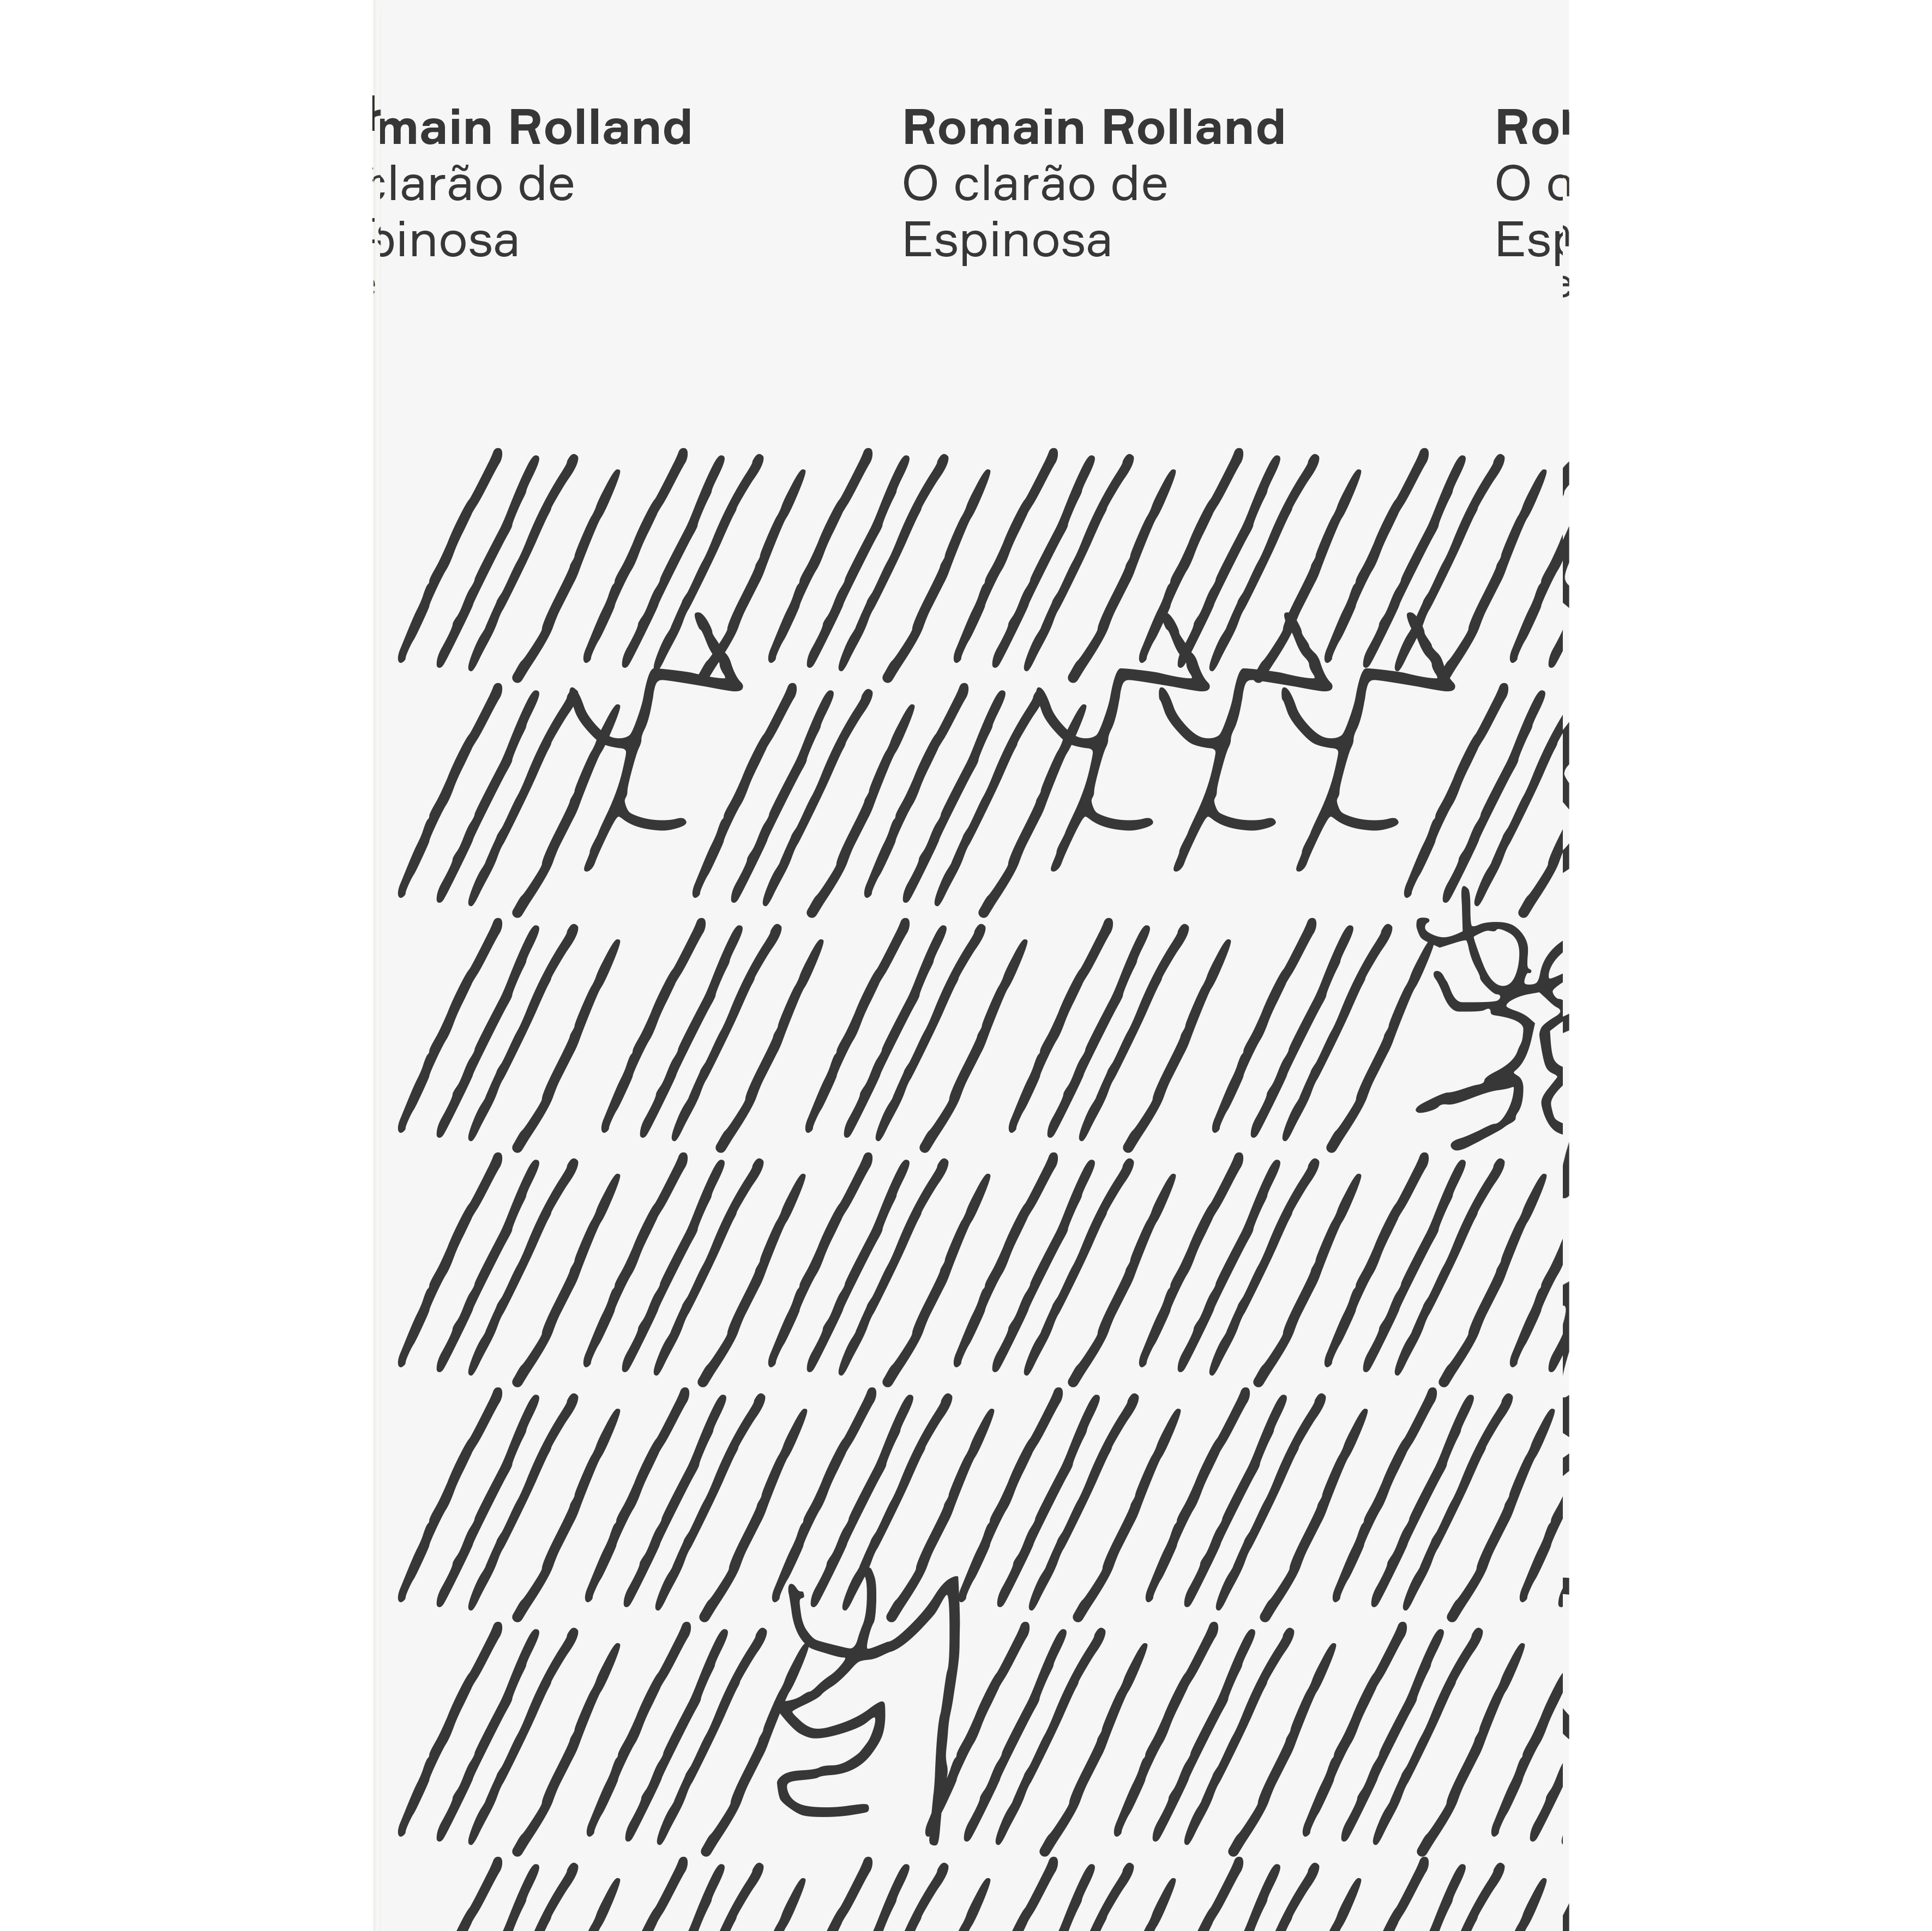
\includegraphics[width=74mm]{./grid/rolland.png}
\end{center}

\hspace*{-7cm}\hrulefill\hspace*{-7cm}

\medskip

\noindent{}Romain Rolland foi novelista, biógrafo, músico e Nobel francês de 1915. Escreveu as presentes páginas sobre Espinosa, repletas de lirismo e potência filosófica, ainda na adolescência, mas foram publicadas apenas em 1942 no livro {\slsc{A viagem interior}}. \hlc[lightyellow]{Neste livro o jovem Rolland conta o “clarão” que teve em sua vida ao ler Espinosa pela primeira vez aos 16 anos, e como isso definiu sua vida e carreira.}

Em cuidadosa edição bilíngue, o leitor aproxima"-se dos movimentos luminosos do texto original. O livro é marcado por uma linguagem fremente e impressionista, que segue rente à experiência de deslumbre e atordoamento de Rolland diante da leitura do filósofo. Por trás das imagens poéticas, vislumbra"-se ainda um questionamento existencial e ontológico da condição humana --- reminiscências da filosofia de Espinosa no pensamento e em sua própria prosa. Como escreve o autor, a leitura de Espinosa foi um “desses jatos da alma, desses clarões, que inundaram minhas veias com o fogo que faz bater o coração do universo”. Às “palavras de fogo de Espinosa” dedica"-se esse relato.

\vfill

\hspace*{-.4cm}\begin{minipage}[c]{.5\linewidth}
\small{
{\Formular{\textbf{
\hspace*{-.1cm}\hlc[lightyellow]{Editora: n-1 \& Hedra}\\
Título: O clarão de Espinosa [bilíngue]\\
Autor: Romain Rolland\\ 
ISBN: 978-65-8109-708-0\\
Páginas: 57\\
Formato: 11x18cm\\
Preço: R\$ 29,90\\
Disponibilidade: 11/09/2020
}}}}
\end{minipage}

\pagebreak

\begin{center}
\hspace*{.5cm}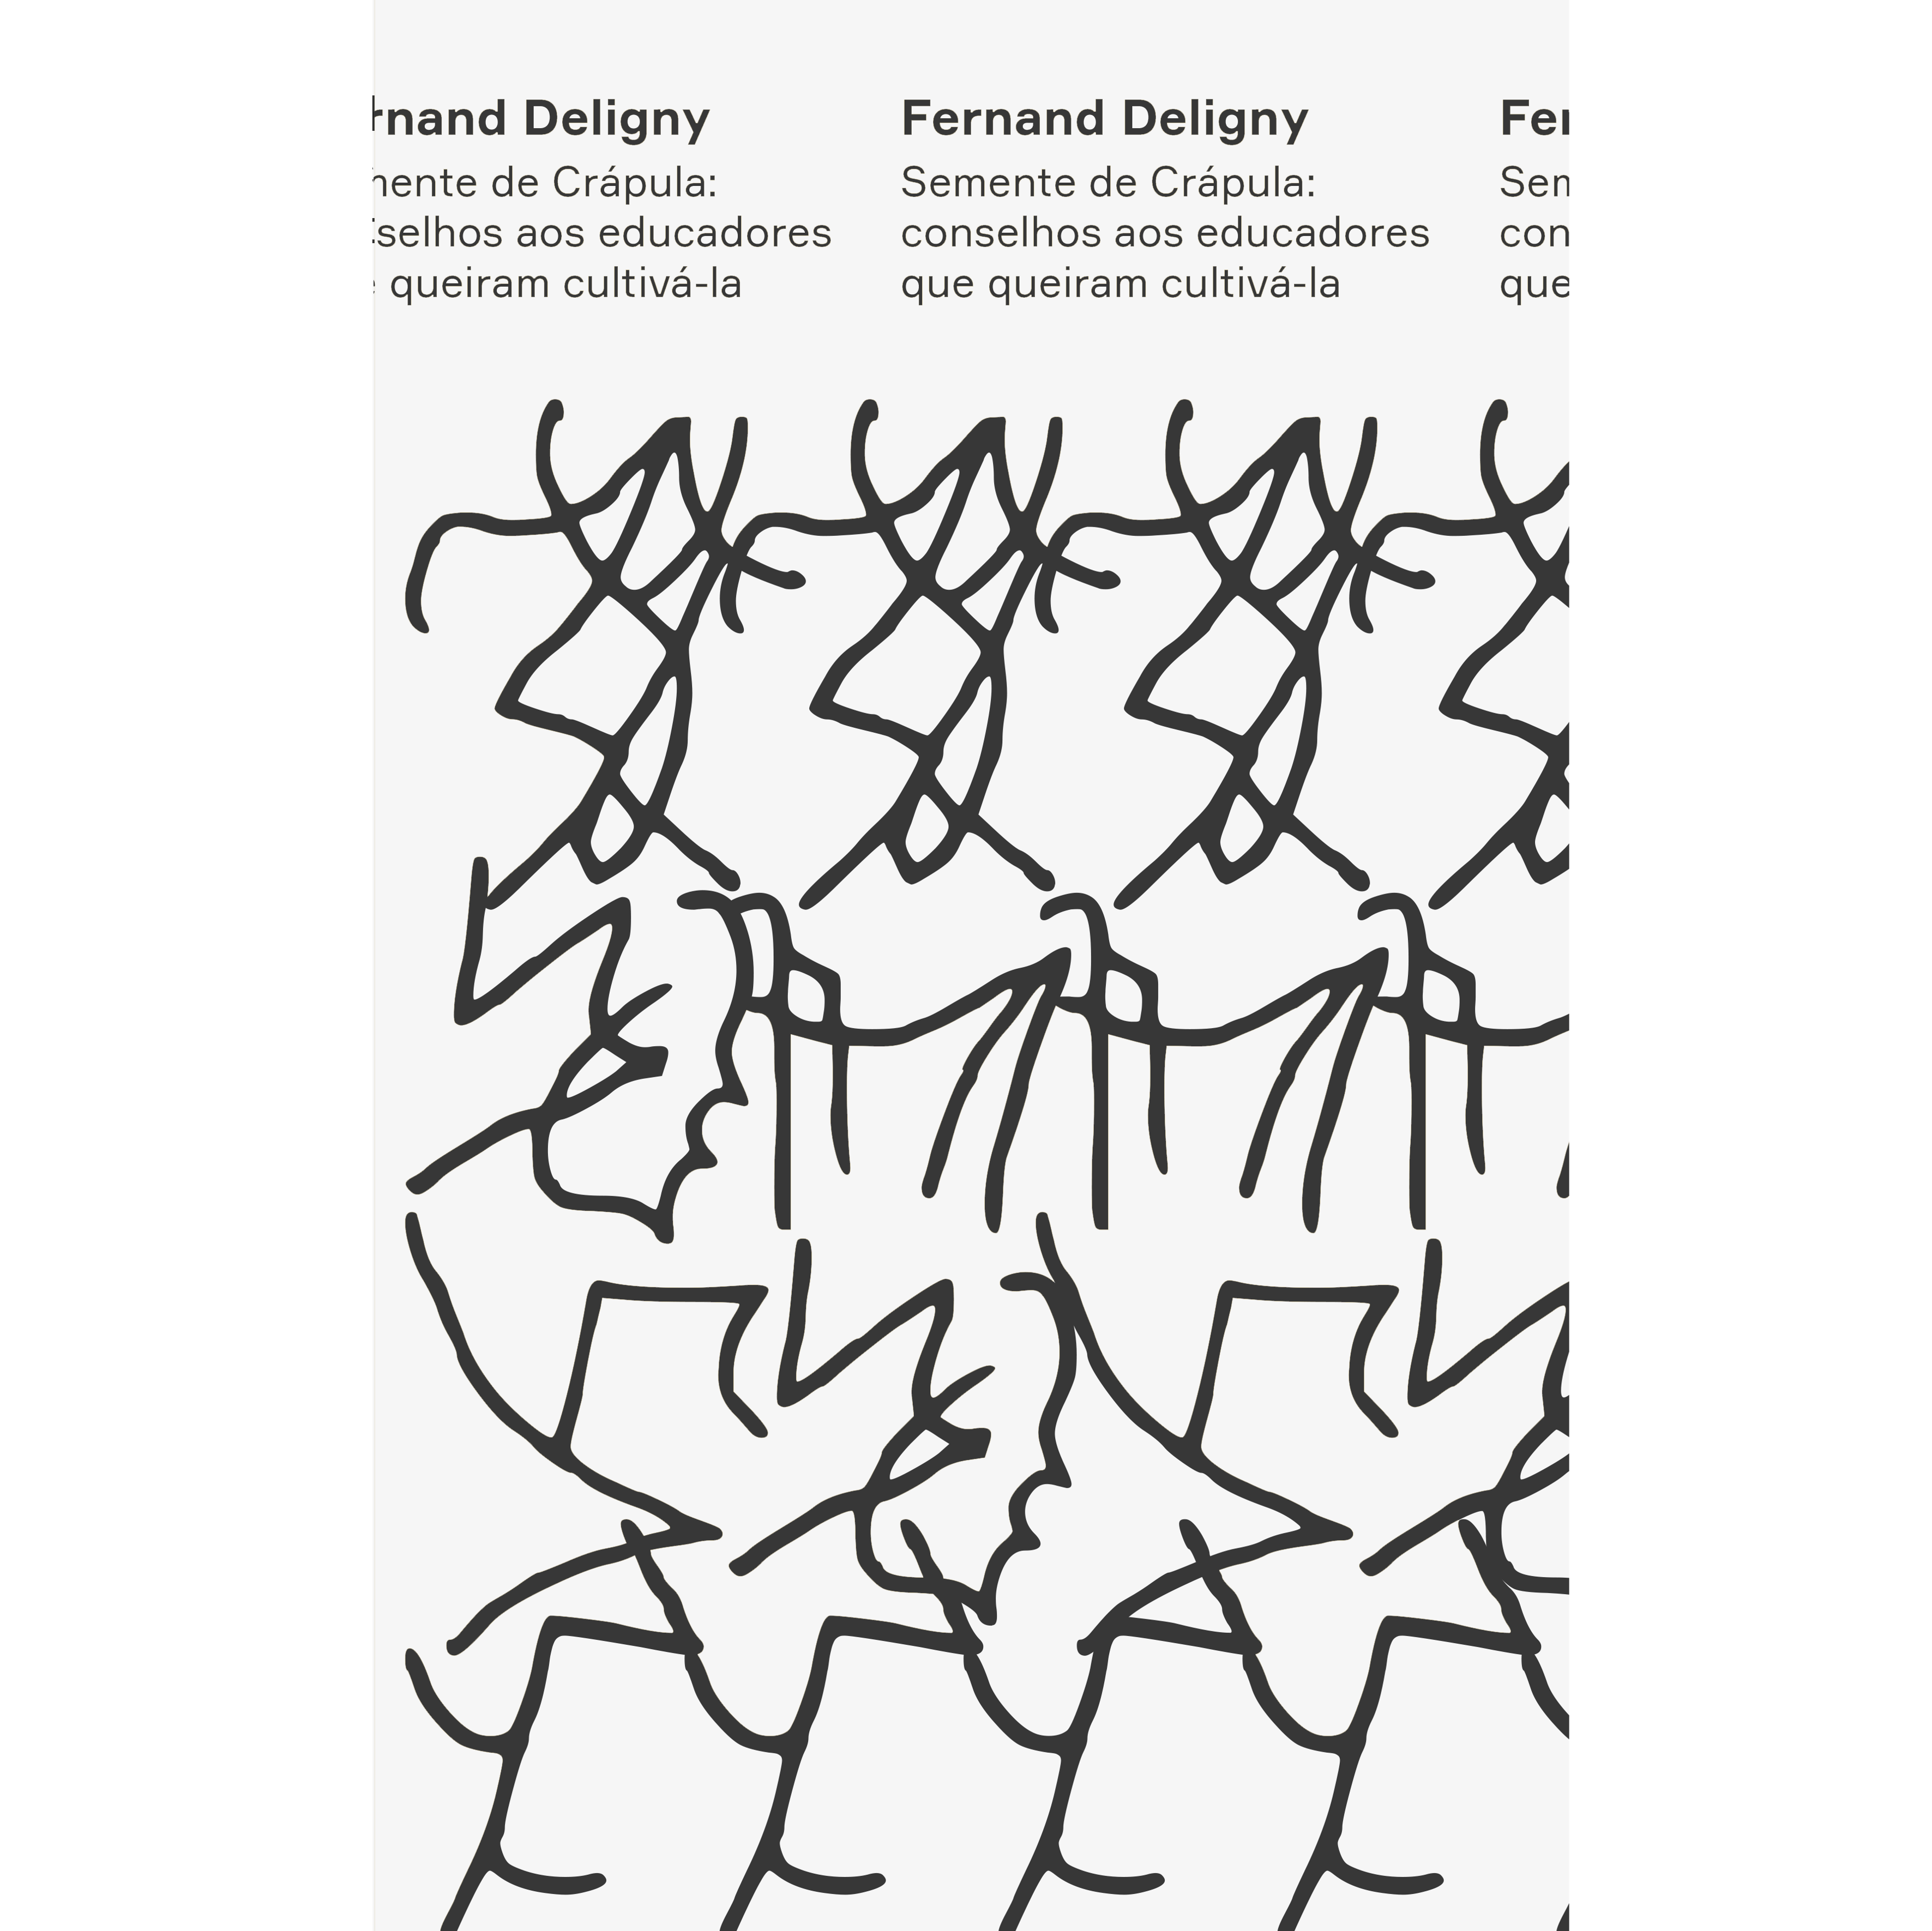
\includegraphics[width=74mm]{./grid/deligny.png}
\end{center}

\hspace*{-7cm}\hrulefill\hspace*{-7cm}

\medskip

\noindent{}{\slsc{Semente de crápula. Conselhos aos educadores que gostariam de cultivá-la}} é o \hlc[lightyellow]{primeiro livro do educador e poeta francês Fernand Deligny. É um balizador de seu trabalho, que o situaria como uma das maiores referências da educação especial} --- lidando com crianças e jovens psicóticos, delinquentes, “perigosos”, “marginais” --- e da pedagogia em geral.

Ao longo dos 134 aforismos, Deligny apresenta suas “sementes”: jovens de um meio social delinquente, cultivadas pelo educador que deve deixar de lutar contra as ervas daninhas, pragas sociais atadas ao nosso convívio social, para mergulhar nas dinâmicas espaciais desses jovens que criam outros sentidos de lugar e convivência no território. Publicado em 1945, o livro foi rapidamente bem sucedido na França por sua linguagem poética simples e a franqueza do autor. Deligny passou os primeiros vinte anos de atuação profissional entre escolas especiais, instituições médico"-pedagógicas e hospitais psiquiátricos.

\vfill

\hspace*{-.4cm}\begin{minipage}[c]{1\linewidth}
\small{
{\Formular{\textbf{
\hspace*{-.1cm}\hlc[lightyellow]{Editora: n-1 \& Hedra}\\
Título: Semente de crápula. Conselhos aos\\ educadores que gostariam de cultivá-la\\
Autor: Fernand Deligny\\ 
ISBN: 978-65-8109-709-7\\
Páginas: 96\\
Formato: 11x18cm\\
Preço: R\$ 34,90\\
Disponibilidade: 11/09/2020
}}}}
\end{minipage}


\pagebreak
\pagestyle{n-1cat}

\begin{multicols}{2}
\begin{enumerate}
\raggedright\nohyphens{
\item Pandemia - Rexistir, {\Formular{\textbf{Eduardo Viveiros de Castro; Achille Mbembe; Carmem Silva; Antonio Negri; Cristina Ribas; Jean Tible; Tatiana Nascimento; Tiqqun; Eduardo Passos; Danichi Hausen Mizoguchi; Yuk Hui}}}
\item Potências do tempo, {\Formular{\textbf{David Lapoujade}}}
\item Declaração, {\Formular{\textbf{Antonio Negri; Michael Hardt}}}
\item Manifesto contrassexual, {\Formular{\textbf{Beatriz Preciado}}}
\item O aracniano e outros textos, {\Formular{\textbf{Fernand Deligny}}}
\item Deleuze, os movimentos aberrantes, {\Formular{\textbf{David Lapoujade}}}
\item Aos nossos amigos, {\Formular{\textbf{Comitê Invisível}}}
\item Teoria King Kong, {\Formular{\textbf{Virginie Despentes}}}
\item Guattari, {\Formular{\textbf{Kuniichi Uno; Laymert Garcia dos Santos}}}
\item Quando e como eu li Foucault, {\Formular{\textbf{Antonio Negri}}}
\item O avesso do niilismo, {\Formular{\textbf{Peter Pál Pelbart}}}
\item A missão, {\Formular{\textbf{Heiner Müller}}}
\item William James, a construção da experiência, {\Formular{\textbf{David Lapoujade}}}
\item Nietzsche -- O bufão dos deuses, {\Formular{\textbf{Maria Cristina Franco Ferraz}}}
\item Impressões de Michel Foucault, {\Formular{\textbf{Roberto Machado}}}
\item Fabulações do corpo japonês, {\Formular{\textbf{Christine Greiner}}}
\item As existências mínimas, {\Formular{\textbf{David Lapoujade}}}
\item Hegel e o Haiti, {\Formular{\textbf{Susan Buck-Morss}}}
\item Brazuca, negão e sebento, {\Formular{\textbf{Jean-Christophe Goddard}}}
\item Motim e destituição agora, {\Formular{\textbf{Comitê Invisível}}}
\item Crítica da razão negra, {\Formular{\textbf{Achille Mbembe}}}
\item Testo junkie, {\Formular{\textbf{Paul B. Preciado}}}
\item O universo inacabado, {\Formular{\textbf{Mario Novello}}}
\item Cartas e outros textos, {\Formular{\textbf{Gilles Deleuze}}}
\item Nietzsche e a filosofia, {\Formular{\textbf{Gilles Deleuze}}}
\item Hijikata tatsumi, {\Formular{\textbf{Kuniichi Uno}}}
\item Spartakus, {\Formular{\textbf{Furio Jesi}}}
\item Agamben, {\Formular{\textbf{Giacoia Jr., Oswaldo}}}
\item UPP -- A redução da favela em três letras, {\Formular{\textbf{Marielle Franco}}}
\item Cinco dias em março, {\Formular{\textbf{Toshiki Okada}}}
\item Os vagabundos eficazes, {\Formular{\textbf{Fernand Deligny}}}
\item O enigma da revolta, {\Formular{\textbf{Michel Foucault}}}
\item Arqueofeminismo
\item Contribuição para a guerra em curso, {\Formular{\textbf{Tiqqun}}}
\item Ética bixa, {\Formular{\textbf{Paco Vidarte}}}
\item Ensaios do assombro, {\Formular{\textbf{Peter Pál Pelbart}}}
\item Metafísicas canibais, {\Formular{\textbf{Eduardo Viveiros de Castro}}}
\item O governo do homem endividado, {\Formular{\textbf{Maurizio Lazzarato}}}
\item Leituras do corpo no Japão, {\Formular{\textbf{Christine Greiner}}}
\item Pragmatismo pulsional, {\Formular{\textbf{João Perci Schiavon}}}
\item Ruptura, {\Formular{\textbf{Centelha}}}
\item Às voltas com Lautréamont, {\Formular{\textbf{Laymert Garcia dos Santos}}}
\item Afrotopia, {\Formular{\textbf{Felwine Sarr}}}
\item Fascismo ou revolução?, {\Formular{\textbf{Maurizio Lazzarato}}}
\item Corpos que importam, {\Formular{\textbf{Judith Butler}}}
\item Somos nosso cérebro?, {\Formular{\textbf{Francisco Ortega; Fernando Vidal}}}
\item Ritornelos, {\Formular{\textbf{Félix Guattari}}}
\item Contracultura, entre a curtição e o experimental, {\Formular{\textbf{Celso Favaretto}}}
}
\end{enumerate}
\end{multicols}

\pagebreak